% Options for packages loaded elsewhere
\PassOptionsToPackage{unicode}{hyperref}
\PassOptionsToPackage{hyphens}{url}
\PassOptionsToPackage{dvipsnames,svgnames,x11names}{xcolor}
%
\documentclass[
  letterpaper,
  DIV=11,
  numbers=noendperiod]{scrartcl}

\usepackage{amsmath,amssymb}
\usepackage{lmodern}
\usepackage{iftex}
\ifPDFTeX
  \usepackage[T1]{fontenc}
  \usepackage[utf8]{inputenc}
  \usepackage{textcomp} % provide euro and other symbols
\else % if luatex or xetex
  \usepackage{unicode-math}
  \defaultfontfeatures{Scale=MatchLowercase}
  \defaultfontfeatures[\rmfamily]{Ligatures=TeX,Scale=1}
\fi
% Use upquote if available, for straight quotes in verbatim environments
\IfFileExists{upquote.sty}{\usepackage{upquote}}{}
\IfFileExists{microtype.sty}{% use microtype if available
  \usepackage[]{microtype}
  \UseMicrotypeSet[protrusion]{basicmath} % disable protrusion for tt fonts
}{}
\makeatletter
\@ifundefined{KOMAClassName}{% if non-KOMA class
  \IfFileExists{parskip.sty}{%
    \usepackage{parskip}
  }{% else
    \setlength{\parindent}{0pt}
    \setlength{\parskip}{6pt plus 2pt minus 1pt}}
}{% if KOMA class
  \KOMAoptions{parskip=half}}
\makeatother
\usepackage{xcolor}
\setlength{\emergencystretch}{3em} % prevent overfull lines
\setcounter{secnumdepth}{-\maxdimen} % remove section numbering
% Make \paragraph and \subparagraph free-standing
\ifx\paragraph\undefined\else
  \let\oldparagraph\paragraph
  \renewcommand{\paragraph}[1]{\oldparagraph{#1}\mbox{}}
\fi
\ifx\subparagraph\undefined\else
  \let\oldsubparagraph\subparagraph
  \renewcommand{\subparagraph}[1]{\oldsubparagraph{#1}\mbox{}}
\fi

\usepackage{color}
\usepackage{fancyvrb}
\newcommand{\VerbBar}{|}
\newcommand{\VERB}{\Verb[commandchars=\\\{\}]}
\DefineVerbatimEnvironment{Highlighting}{Verbatim}{commandchars=\\\{\}}
% Add ',fontsize=\small' for more characters per line
\usepackage{framed}
\definecolor{shadecolor}{RGB}{241,243,245}
\newenvironment{Shaded}{\begin{snugshade}}{\end{snugshade}}
\newcommand{\AlertTok}[1]{\textcolor[rgb]{0.68,0.00,0.00}{#1}}
\newcommand{\AnnotationTok}[1]{\textcolor[rgb]{0.37,0.37,0.37}{#1}}
\newcommand{\AttributeTok}[1]{\textcolor[rgb]{0.40,0.45,0.13}{#1}}
\newcommand{\BaseNTok}[1]{\textcolor[rgb]{0.68,0.00,0.00}{#1}}
\newcommand{\BuiltInTok}[1]{\textcolor[rgb]{0.00,0.23,0.31}{#1}}
\newcommand{\CharTok}[1]{\textcolor[rgb]{0.13,0.47,0.30}{#1}}
\newcommand{\CommentTok}[1]{\textcolor[rgb]{0.37,0.37,0.37}{#1}}
\newcommand{\CommentVarTok}[1]{\textcolor[rgb]{0.37,0.37,0.37}{\textit{#1}}}
\newcommand{\ConstantTok}[1]{\textcolor[rgb]{0.56,0.35,0.01}{#1}}
\newcommand{\ControlFlowTok}[1]{\textcolor[rgb]{0.00,0.23,0.31}{#1}}
\newcommand{\DataTypeTok}[1]{\textcolor[rgb]{0.68,0.00,0.00}{#1}}
\newcommand{\DecValTok}[1]{\textcolor[rgb]{0.68,0.00,0.00}{#1}}
\newcommand{\DocumentationTok}[1]{\textcolor[rgb]{0.37,0.37,0.37}{\textit{#1}}}
\newcommand{\ErrorTok}[1]{\textcolor[rgb]{0.68,0.00,0.00}{#1}}
\newcommand{\ExtensionTok}[1]{\textcolor[rgb]{0.00,0.23,0.31}{#1}}
\newcommand{\FloatTok}[1]{\textcolor[rgb]{0.68,0.00,0.00}{#1}}
\newcommand{\FunctionTok}[1]{\textcolor[rgb]{0.28,0.35,0.67}{#1}}
\newcommand{\ImportTok}[1]{\textcolor[rgb]{0.00,0.46,0.62}{#1}}
\newcommand{\InformationTok}[1]{\textcolor[rgb]{0.37,0.37,0.37}{#1}}
\newcommand{\KeywordTok}[1]{\textcolor[rgb]{0.00,0.23,0.31}{#1}}
\newcommand{\NormalTok}[1]{\textcolor[rgb]{0.00,0.23,0.31}{#1}}
\newcommand{\OperatorTok}[1]{\textcolor[rgb]{0.37,0.37,0.37}{#1}}
\newcommand{\OtherTok}[1]{\textcolor[rgb]{0.00,0.23,0.31}{#1}}
\newcommand{\PreprocessorTok}[1]{\textcolor[rgb]{0.68,0.00,0.00}{#1}}
\newcommand{\RegionMarkerTok}[1]{\textcolor[rgb]{0.00,0.23,0.31}{#1}}
\newcommand{\SpecialCharTok}[1]{\textcolor[rgb]{0.37,0.37,0.37}{#1}}
\newcommand{\SpecialStringTok}[1]{\textcolor[rgb]{0.13,0.47,0.30}{#1}}
\newcommand{\StringTok}[1]{\textcolor[rgb]{0.13,0.47,0.30}{#1}}
\newcommand{\VariableTok}[1]{\textcolor[rgb]{0.07,0.07,0.07}{#1}}
\newcommand{\VerbatimStringTok}[1]{\textcolor[rgb]{0.13,0.47,0.30}{#1}}
\newcommand{\WarningTok}[1]{\textcolor[rgb]{0.37,0.37,0.37}{\textit{#1}}}

\providecommand{\tightlist}{%
  \setlength{\itemsep}{0pt}\setlength{\parskip}{0pt}}\usepackage{longtable,booktabs,array}
\usepackage{calc} % for calculating minipage widths
% Correct order of tables after \paragraph or \subparagraph
\usepackage{etoolbox}
\makeatletter
\patchcmd\longtable{\par}{\if@noskipsec\mbox{}\fi\par}{}{}
\makeatother
% Allow footnotes in longtable head/foot
\IfFileExists{footnotehyper.sty}{\usepackage{footnotehyper}}{\usepackage{footnote}}
\makesavenoteenv{longtable}
\usepackage{graphicx}
\makeatletter
\def\maxwidth{\ifdim\Gin@nat@width>\linewidth\linewidth\else\Gin@nat@width\fi}
\def\maxheight{\ifdim\Gin@nat@height>\textheight\textheight\else\Gin@nat@height\fi}
\makeatother
% Scale images if necessary, so that they will not overflow the page
% margins by default, and it is still possible to overwrite the defaults
% using explicit options in \includegraphics[width, height, ...]{}
\setkeys{Gin}{width=\maxwidth,height=\maxheight,keepaspectratio}
% Set default figure placement to htbp
\makeatletter
\def\fps@figure{htbp}
\makeatother

\KOMAoption{captions}{tableheading}
\makeatletter
\makeatother
\makeatletter
\makeatother
\makeatletter
\@ifpackageloaded{caption}{}{\usepackage{caption}}
\AtBeginDocument{%
\ifdefined\contentsname
  \renewcommand*\contentsname{Table of contents}
\else
  \newcommand\contentsname{Table of contents}
\fi
\ifdefined\listfigurename
  \renewcommand*\listfigurename{List of Figures}
\else
  \newcommand\listfigurename{List of Figures}
\fi
\ifdefined\listtablename
  \renewcommand*\listtablename{List of Tables}
\else
  \newcommand\listtablename{List of Tables}
\fi
\ifdefined\figurename
  \renewcommand*\figurename{Figure}
\else
  \newcommand\figurename{Figure}
\fi
\ifdefined\tablename
  \renewcommand*\tablename{Table}
\else
  \newcommand\tablename{Table}
\fi
}
\@ifpackageloaded{float}{}{\usepackage{float}}
\floatstyle{ruled}
\@ifundefined{c@chapter}{\newfloat{codelisting}{h}{lop}}{\newfloat{codelisting}{h}{lop}[chapter]}
\floatname{codelisting}{Listing}
\newcommand*\listoflistings{\listof{codelisting}{List of Listings}}
\makeatother
\makeatletter
\@ifpackageloaded{caption}{}{\usepackage{caption}}
\@ifpackageloaded{subcaption}{}{\usepackage{subcaption}}
\makeatother
\makeatletter
\@ifpackageloaded{tcolorbox}{}{\usepackage[many]{tcolorbox}}
\makeatother
\makeatletter
\@ifundefined{shadecolor}{\definecolor{shadecolor}{rgb}{.97, .97, .97}}
\makeatother
\makeatletter
\makeatother
\ifLuaTeX
  \usepackage{selnolig}  % disable illegal ligatures
\fi
\IfFileExists{bookmark.sty}{\usepackage{bookmark}}{\usepackage{hyperref}}
\IfFileExists{xurl.sty}{\usepackage{xurl}}{} % add URL line breaks if available
\urlstyle{same} % disable monospaced font for URLs
\hypersetup{
  pdftitle={Lefty Lemurs},
  colorlinks=true,
  linkcolor={blue},
  filecolor={Maroon},
  citecolor={Blue},
  urlcolor={Blue},
  pdfcreator={LaTeX via pandoc}}

\title{Lefty Lemurs}
\author{}
\date{}

\begin{document}
\maketitle
\ifdefined\Shaded\renewenvironment{Shaded}{\begin{tcolorbox}[frame hidden, sharp corners, interior hidden, borderline west={3pt}{0pt}{shadecolor}, breakable, enhanced, boxrule=0pt]}{\end{tcolorbox}}\fi

Loading library

\begin{Shaded}
\begin{Highlighting}[]
\FunctionTok{library}\NormalTok{(tidyverse)}
\end{Highlighting}
\end{Shaded}

\begin{verbatim}
-- Attaching packages --------------------------------------- tidyverse 1.3.1 --
\end{verbatim}

\begin{verbatim}
v ggplot2 3.3.6     v purrr   0.3.4
v tibble  3.1.7     v dplyr   1.0.9
v tidyr   1.2.0     v stringr 1.4.0
v readr   2.1.2     v forcats 0.5.1
\end{verbatim}

\begin{verbatim}
-- Conflicts ------------------------------------------ tidyverse_conflicts() --
x dplyr::filter() masks stats::filter()
x dplyr::lag()    masks stats::lag()
\end{verbatim}

\begin{Shaded}
\begin{Highlighting}[]
\FunctionTok{library}\NormalTok{(readr)}
\FunctionTok{library}\NormalTok{(dplyr)}
\FunctionTok{library}\NormalTok{(ggplot2)}
\end{Highlighting}
\end{Shaded}

\textbf{Here's what I did to clean the data:}

Importing dataset

\begin{Shaded}
\begin{Highlighting}[]
\NormalTok{L\_PreClean }\OtherTok{\textless{}{-}} \FunctionTok{read.csv}\NormalTok{(}\StringTok{"\textasciitilde{}/Documents/GitHub/Lefty\_Lemurs/LeftyLemurs\_Original.csv"}\NormalTok{)}
\end{Highlighting}
\end{Shaded}

\begin{Shaded}
\begin{Highlighting}[]
\FunctionTok{summary}\NormalTok{(L\_PreClean)}
\end{Highlighting}
\end{Shaded}

\begin{verbatim}
 Troop.............A..B..C..D.... Focal.Lemur          Species         
 Length:694                       Length:694         Length:694        
 Class :character                 Class :character   Class :character  
 Mode  :character                 Mode  :character   Mode  :character  
                                                                       
                                                                       
                                                                       
     Sex                Month            Day             Year     
 Length:694         Min.   :6.000   Min.   : 1.00   Min.   :2022  
 Class :character   1st Qu.:6.000   1st Qu.: 8.00   1st Qu.:2022  
 Mode  :character   Median :6.000   Median :22.00   Median :2022  
                    Mean   :6.411   Mean   :18.29   Mean   :2022  
                    3rd Qu.:7.000   3rd Qu.:28.00   3rd Qu.:2022  
                    Max.   :7.000   Max.   :30.00   Max.   :2022  
 Time..H.M.S.         Category        
 Length:694         Length:694        
 Class :character   Class :character  
 Mode  :character   Mode  :character  
                                      
                                      
                                      
 Focal.sample.note......................................................................................................................................................please.include.as.much.detail.as.possible...If.a.note.is.about.a.grooming.bout..for.example..include.stop.time.in.the.same.cell.
 Length:694                                                                                                                                                                                                                                                                                             
 Class :character                                                                                                                                                                                                                                                                                       
 Mode  :character                                                                                                                                                                                                                                                                                       
                                                                                                                                                                                                                                                                                                        
                                                                                                                                                                                                                                                                                                        
                                                                                                                                                                                                                                                                                                        
\end{verbatim}

rename long column names to simpler ones

\begin{Shaded}
\begin{Highlighting}[]
\NormalTok{L\_PreClean }\OtherTok{\textless{}{-}} \FunctionTok{rename}\NormalTok{(L\_PreClean, }\AttributeTok{Troop =}\NormalTok{ Troop.............A..B..C..D...., }\AttributeTok{Time =}\NormalTok{ Time..H.M.S., }\AttributeTok{Note =}\NormalTok{ Focal.sample.note......................................................................................................................................................please.include.as.much.detail.as.possible...If.a.note.is.about.a.grooming.bout..for.example..include.stop.time.in.the.same.cell.)}
\end{Highlighting}
\end{Shaded}

remove commas in the category column

\begin{Shaded}
\begin{Highlighting}[]
\NormalTok{L\_PreClean}\SpecialCharTok{$}\NormalTok{Category }\OtherTok{\textless{}{-}} \FunctionTok{str\_replace}\NormalTok{(L\_PreClean}\SpecialCharTok{$}\NormalTok{Category, }\StringTok{","}\NormalTok{, }\StringTok{""}\NormalTok{)}
\end{Highlighting}
\end{Shaded}

Why on earth did it make it into a value instead of a new data frame???
I guess it doesn't matter because it still works\ldots{}

Sometimes I wrote behaviors in all caps, and sometimes I didn't. I'm
just going to put all of them in all caps because it's easier.

\begin{Shaded}
\begin{Highlighting}[]
\NormalTok{L\_PreClean}\SpecialCharTok{$}\NormalTok{Category }\OtherTok{=} \FunctionTok{toupper}\NormalTok{(L\_PreClean}\SpecialCharTok{$}\NormalTok{Category)}
\end{Highlighting}
\end{Shaded}

I have some data where I didn't actually record the limb used. Why did I
do that? I'm going to delete the rows where I forgot to list the limb.

Only keep rows in categories that don't contain RH, LH, RF, and/or LF

\begin{Shaded}
\begin{Highlighting}[]
\NormalTok{L\_HFdata }\OtherTok{\textless{}{-}}
\NormalTok{  L\_PreClean }\SpecialCharTok{\%\textgreater{}\%}
  \FunctionTok{filter}\NormalTok{(}\FunctionTok{str\_detect}\NormalTok{(Category, }\StringTok{"RH|RF|LH|LF"}\NormalTok{))}
\end{Highlighting}
\end{Shaded}

Squeaky clean

Now I want to create a separate data frame that only contains behaviors
from my ethogram:

\begin{Shaded}
\begin{Highlighting}[]
\CommentTok{\# do not run }
\CommentTok{\# lefty\_justEthogram \textless{}{-}}
\CommentTok{\# L \%\textgreater{}\%  select(Category) \%\textgreater{}\%}
\CommentTok{\# filter(str\_detect(Category, "BP|QP|L|AG|SG|F|E|CL|HC|R|G|"))}
\end{Highlighting}
\end{Shaded}

Why didn't it work

\emph{This did not work} Would it be possible to split the ``Category''
column into 2 columns? 1 that says ``Task'' and another that says
``Limb''?

``Limb'' would have LH/RH/LF/RH and ``Task'' would have the other stuff

I think if I duplicate the column and rename it and then eliminate the
limbs from ``Task'' and keep only the limbs in ``Limbs'' it might work.

Then I can rename the tasks to ``Eating/Grooming/Locomotion/etc.

Duplicating ``Category'' and calling the new one ``Limb''

\begin{Shaded}
\begin{Highlighting}[]
\CommentTok{\# do not run: L\_HFdata$Limb \textless{}{-} L\_PreClean$Category}
\CommentTok{\# do not run: L\_PreClean2 \textless{}{-} L\_PreClean \%\textgreater{}\% relocate (Limb, .before = Note)}
\end{Highlighting}
\end{Shaded}

\emph{This did not work}

Replacing limb with nothing

\begin{Shaded}
\begin{Highlighting}[]
\CommentTok{\# do not run: lefty\_split \textless{}{-} L\_PreClean2$Category \textless{}{-} str\_replace(L\_PreClean$Limb, "BP|QP|L|AG|SG|F|E|CL|HC|R|G|", "")}

\CommentTok{\# do not run: lefty\_fullsplit \textless{}{-} L\_PreClean2$Limb \textless{}{-} str\_replace(L\_PreClean$Category, "LF|LH|RF|RH|", "")}
\end{Highlighting}
\end{Shaded}

Categories kept limbs because they include an R (like rest) or L (like
locomotion) I think limb section stayed the same? I think it kept all
the columns that contained the limbs, which was all of them ofc. I might
be running the wrong code.

Okay I'm going to use find and replace in Excel to fix it because R
doesn't know how to do anything apparently and I literally want to cry
rn

Wait wtf why does it say 30,000+ rows columns

\hypertarget{okay-ive-spent-4-hours-trying-to-get-it-to-work-and-tbh-this-is-a-waste-of-time-so-im-just-going-to-export-the-behavior-data-as-a-csv-and-finish-cleaning-it-in-google-sheets}{%
\subsection{okay I've spent 4 hours trying to get it to work and tbh
this is a waste of time so I'm just going to export the behavior data as
a CSV and finish cleaning it in Google
Sheets}\label{okay-ive-spent-4-hours-trying-to-get-it-to-work-and-tbh-this-is-a-waste-of-time-so-im-just-going-to-export-the-behavior-data-as-a-csv-and-finish-cleaning-it-in-google-sheets}}

Writing as CSV bc my attempts at making limb column completely failed
after working on it for 2 days

\begin{Shaded}
\begin{Highlighting}[]
\CommentTok{\# write\_csv(L\_PreClean,"Lefty\_Lemurs.csv")}
\end{Highlighting}
\end{Shaded}

\begin{center}\rule{0.5\linewidth}{0.5pt}\end{center}

\textbf{Here's what I did in Google Sheets with the CSV file} (I really
wanted to do it in R but I could not figure it out and wasted hours and
hours)

\begin{itemize}
\tightlist
\item
  Deleted rows that didn't contain behaviors from my ethogram
\item
  Copied ``Category'' into 2 columns
\item
  In old Category column, deleted limb data
\item
  In new ``Limb'' data, kept only limb data (not behavior)
\item
  Deleted rows that had question marks in data
\item
  Deleted data where category was ``Other''
\item
  Deleted data that had rows with both hands
\item
  Merged ``F'' and ``E'' into one category ``E''
\item
  Looked through notes to change category when it was just ``G''. Most
  got changed to L, some got changed to R, a few got deleted
\item
  Added new column for H/F to say whether limb was hand or foot
\item
  Added new column for side to say whether limb was left or right
\end{itemize}

New categories - E (eating/foraging) - R (resting) (lemur is still) - L
(locomotion) (active motion like leaping, climbing, or jumping) - CL
(cross legs) - HC (hand clasp) - BP (bipedal walking) - QP (quadrupedal
walking) - LA (land) - SG (self grooming) - AG (allo-grooming)

\textbf{\emph{Upload clean data}} (it was a nightmare of cleaning this
data in R and Excel and took many terrible hours, of which I do not wish
to relive)

\begin{Shaded}
\begin{Highlighting}[]
\NormalTok{L }\OtherTok{\textless{}{-}} \FunctionTok{read.csv}\NormalTok{(}\StringTok{"\textasciitilde{}/Documents/GitHub/Lefty\_Lemurs/LeftyLemurs\_Clean.csv"}\NormalTok{)}
\end{Highlighting}
\end{Shaded}

\textbf{Analysis}

\textasciitilde Hex codes for colors (to use in graphs)\textasciitilde{}
Red: \#C84E00 Orange: \#E89923 Yellow: \#FFD960 Light Green: \#A1B70D
Turquoise: \#339898 Teal: \#1D6363 Medium Blue: \#005587 Light Blue:
\#0577B1 Purple: \#993399

\begin{Shaded}
\begin{Highlighting}[]
\FunctionTok{head}\NormalTok{(L)}
\end{Highlighting}
\end{Shaded}

\begin{verbatim}
  Troop    Focal Species Age Sex Month Day Year    Time Category Limb H.F Side
1     P Carolina    Emon  12   F     6  30 2022 8:25:26        E   RH   H    R
2     P Carolina    Emon  12   F     6  30 2022 8:28:29        E   RH   H    R
3     P Carolina    Emon  12   F     6  30 2022 8:23:54        E   LH   H    L
4     P Carolina    Emon  12   F     6  30 2022 8:25:47        E   LH   H    L
5     P Carolina    Emon  12   F     6  30 2022 8:27:13        E   LH   H    L
6     P Carolina    Emon  12   F     6  30 2022 8:43:36        E   LH   H    L
                                              Note
1        Grasp silverberry with right hand and eat
2 Grasp and eat silverberry with right hand on top
3          Grab silverberry with left hand and eat
4         Grasp silverberry with left hand and eat
5   Grasp silverberry plant with left hand and eat
6   Forage and eat evergreen leaves with left hand
\end{verbatim}

Let's look at how many total instances of each limb use there was

\begin{Shaded}
\begin{Highlighting}[]
\FunctionTok{table}\NormalTok{(L}\SpecialCharTok{$}\NormalTok{Limb)}
\end{Highlighting}
\end{Shaded}

\begin{verbatim}

 LF  LH  RF  RH 
 32 225  47 318 
\end{verbatim}

Omg

Left Hand: 225 Right Hand: 318 Left Foot: 32 Right Foot: 47

It looks like lemurs used their right hands a lot more than they used
their left hands\ldots{}

\begin{Shaded}
\begin{Highlighting}[]
 \FunctionTok{ggplot}\NormalTok{ (L, }\FunctionTok{aes}\NormalTok{(}\AttributeTok{x=} \FunctionTok{reorder}\NormalTok{ (Limb, Limb, table ))) }\SpecialCharTok{+}
  \FunctionTok{geom\_bar}\NormalTok{(}\AttributeTok{color =} \StringTok{"black"}\NormalTok{, }\AttributeTok{fill =} \StringTok{"\#012169"}\NormalTok{) }\SpecialCharTok{+}
  \FunctionTok{theme\_classic}\NormalTok{() }\SpecialCharTok{+}
  \FunctionTok{xlab}\NormalTok{(}\StringTok{"Limb"}\NormalTok{) }\SpecialCharTok{+}
  \FunctionTok{ylab}\NormalTok{(}\StringTok{"Total Times Using Each Limb"}\NormalTok{) }\SpecialCharTok{+}
  \FunctionTok{ggtitle}\NormalTok{(}\StringTok{"Total Limb Use Across Lemurs"}\NormalTok{) }\SpecialCharTok{+}
  \FunctionTok{coord\_flip}\NormalTok{()}
\end{Highlighting}
\end{Shaded}

\begin{figure}[H]

{\centering 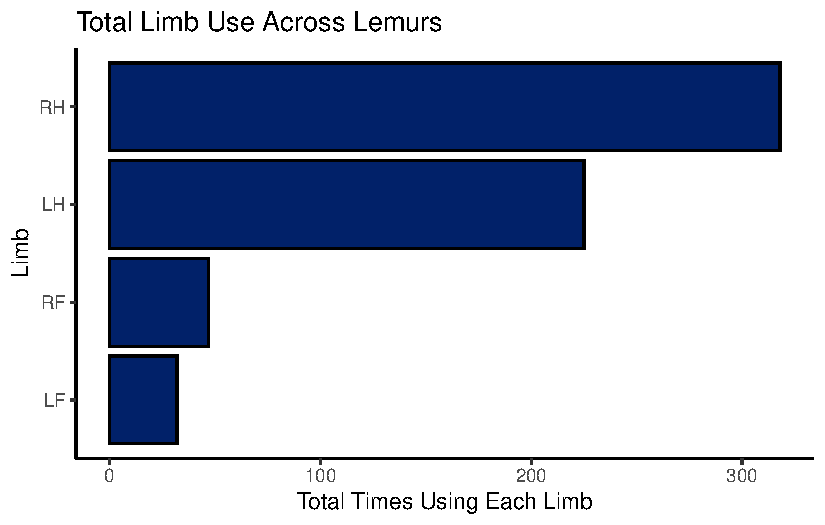
\includegraphics{LeftyLemurs_files/figure-pdf/unnamed-chunk-15-1.pdf}

}

\end{figure}

Yep, there definitely appears to be a hand/foot preference

\begin{Shaded}
\begin{Highlighting}[]
\FunctionTok{ggplot}\NormalTok{ (L, }\FunctionTok{aes}\NormalTok{(}\AttributeTok{x=} \FunctionTok{reorder}\NormalTok{ (Limb, Limb, table ))) }\SpecialCharTok{+}
  \FunctionTok{geom\_bar}\NormalTok{(}\AttributeTok{color =} \StringTok{"black"}\NormalTok{, }\AttributeTok{fill =} \StringTok{"\#C84E00"}\NormalTok{) }\SpecialCharTok{+}
  \FunctionTok{theme\_classic}\NormalTok{() }\SpecialCharTok{+}
  \FunctionTok{xlab}\NormalTok{(}\StringTok{"Limb"}\NormalTok{) }\SpecialCharTok{+}
  \FunctionTok{ylab}\NormalTok{(}\StringTok{"Total Times Using Each Limb"}\NormalTok{) }\SpecialCharTok{+}
  \FunctionTok{ggtitle}\NormalTok{(}\StringTok{"Total Limb Use Across Lemur Species"}\NormalTok{) }\SpecialCharTok{+}
  \FunctionTok{coord\_flip}\NormalTok{() }\SpecialCharTok{+}
  \FunctionTok{facet\_wrap}\NormalTok{ (}\SpecialCharTok{\textasciitilde{}}\NormalTok{ Species, }\AttributeTok{scales =} \StringTok{"free"}\NormalTok{)}
\end{Highlighting}
\end{Shaded}

\begin{figure}[H]

{\centering 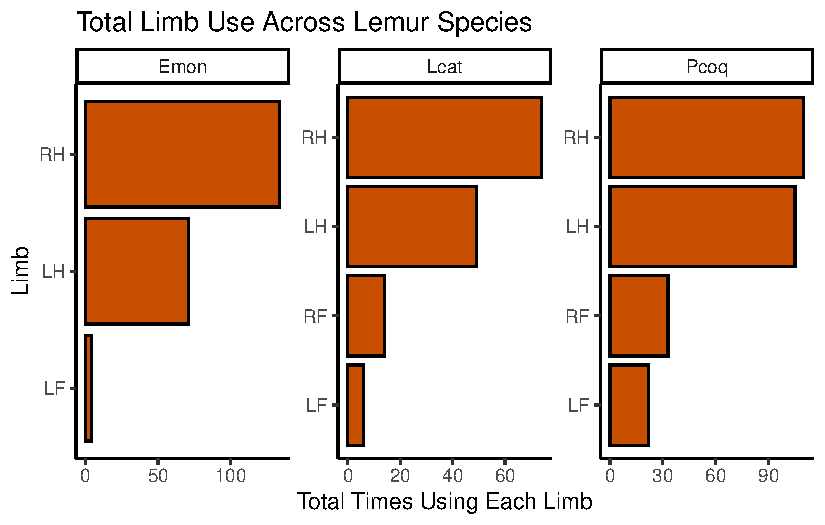
\includegraphics{LeftyLemurs_files/figure-pdf/unnamed-chunk-16-1.pdf}

}

\end{figure}

\begin{Shaded}
\begin{Highlighting}[]
\FunctionTok{ggplot}\NormalTok{ (L, }\FunctionTok{aes}\NormalTok{(}\AttributeTok{x=}\NormalTok{ Side)) }\SpecialCharTok{+}
  \FunctionTok{geom\_bar}\NormalTok{(}\AttributeTok{color =} \StringTok{"black"}\NormalTok{, }\AttributeTok{fill =} \StringTok{"\#C84E00"}\NormalTok{) }\SpecialCharTok{+}
  \FunctionTok{theme\_classic}\NormalTok{() }\SpecialCharTok{+}
  \FunctionTok{xlab}\NormalTok{(}\StringTok{"Left or Right Side"}\NormalTok{) }\SpecialCharTok{+}
  \FunctionTok{ylab}\NormalTok{(}\StringTok{"\# of Times Using Each Limb"}\NormalTok{) }\SpecialCharTok{+}
  \FunctionTok{ggtitle}\NormalTok{(}\StringTok{"Limb Use Between Lemur Species"}\NormalTok{) }\SpecialCharTok{+}
  \FunctionTok{facet\_wrap}\NormalTok{ (}\SpecialCharTok{\textasciitilde{}}\NormalTok{ Species, }\AttributeTok{scales =} \StringTok{"free"}\NormalTok{)}
\end{Highlighting}
\end{Shaded}

\begin{figure}[H]

{\centering 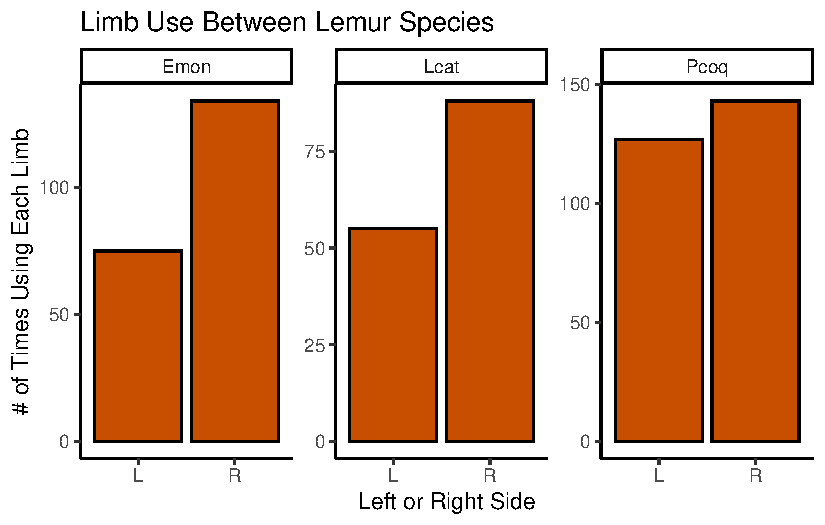
\includegraphics{LeftyLemurs_files/figure-pdf/unnamed-chunk-17-1.pdf}

}

\end{figure}

\begin{Shaded}
\begin{Highlighting}[]
\FunctionTok{ggplot}\NormalTok{ (L, }\FunctionTok{aes}\NormalTok{(}\AttributeTok{x=} \FunctionTok{reorder}\NormalTok{ (Side, Side, table ))) }\SpecialCharTok{+}
  \FunctionTok{geom\_bar}\NormalTok{(}\AttributeTok{color =} \StringTok{"black"}\NormalTok{, }\AttributeTok{fill =} \StringTok{"\#C84E00"}\NormalTok{) }\SpecialCharTok{+}
  \FunctionTok{theme\_classic}\NormalTok{() }\SpecialCharTok{+}
  \FunctionTok{xlab}\NormalTok{(}\StringTok{"Left or Right"}\NormalTok{) }\SpecialCharTok{+}
  \FunctionTok{ylab}\NormalTok{(}\StringTok{"Total Times Using Each Limb"}\NormalTok{) }\SpecialCharTok{+}
  \FunctionTok{ggtitle}\NormalTok{(}\StringTok{"Limb Use Between Lemur Species"}\NormalTok{) }\SpecialCharTok{+}
  \FunctionTok{coord\_flip}\NormalTok{() }\SpecialCharTok{+}
  \FunctionTok{facet\_wrap}\NormalTok{ (}\SpecialCharTok{\textasciitilde{}}\NormalTok{ Species, }\AttributeTok{scales =} \StringTok{"free"}\NormalTok{)}
\end{Highlighting}
\end{Shaded}

\begin{figure}[H]

{\centering 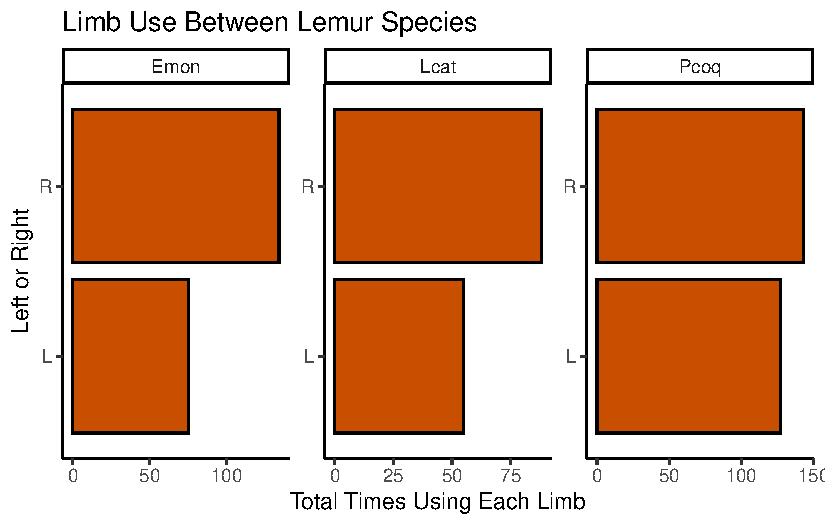
\includegraphics{LeftyLemurs_files/figure-pdf/unnamed-chunk-18-1.pdf}

}

\end{figure}

Same thing but on the same scale (I got more data from sifakas as u can
see)

\begin{Shaded}
\begin{Highlighting}[]
\FunctionTok{ggplot}\NormalTok{ (L, }\FunctionTok{aes}\NormalTok{(}\AttributeTok{x=}\NormalTok{ Side)) }\SpecialCharTok{+}
  \FunctionTok{geom\_bar}\NormalTok{(}\AttributeTok{color =} \StringTok{"black"}\NormalTok{, }\AttributeTok{fill =} \StringTok{"\#C84E00"}\NormalTok{) }\SpecialCharTok{+}
  \FunctionTok{theme\_classic}\NormalTok{() }\SpecialCharTok{+}
  \FunctionTok{xlab}\NormalTok{(}\StringTok{"Left or Right Side"}\NormalTok{) }\SpecialCharTok{+}
  \FunctionTok{ylab}\NormalTok{(}\StringTok{"\# of Times Using Each Limb"}\NormalTok{) }\SpecialCharTok{+}
  \FunctionTok{ggtitle}\NormalTok{(}\StringTok{"Limb Use Between Lemur Species"}\NormalTok{) }\SpecialCharTok{+}
  \FunctionTok{facet\_wrap}\NormalTok{ (}\SpecialCharTok{\textasciitilde{}}\NormalTok{ Species,)}
\end{Highlighting}
\end{Shaded}

\begin{figure}[H]

{\centering 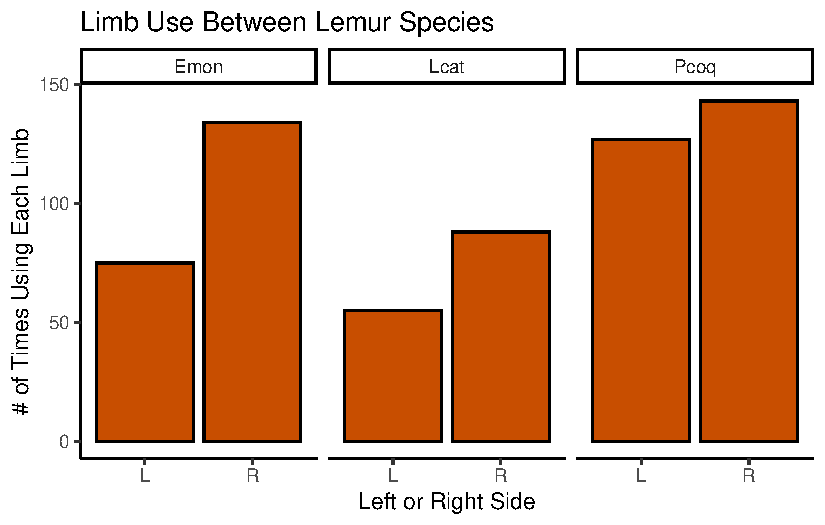
\includegraphics{LeftyLemurs_files/figure-pdf/unnamed-chunk-19-1.pdf}

}

\end{figure}

👀 Sifakas have higher left hand use than the other 2 species. Sifakas
overall seem more ambidextrous. However, this could be due to them
foraging more (maybe all lemurs forage more with their left hands or
something idk). Therefore I should separate it out by eating behaviors.

What about by sex

\begin{Shaded}
\begin{Highlighting}[]
\FunctionTok{ggplot}\NormalTok{ (L, }\FunctionTok{aes}\NormalTok{(}\AttributeTok{x =} \FunctionTok{reorder}\NormalTok{ (Limb, Limb, table ))) }\SpecialCharTok{+}
  \FunctionTok{geom\_bar}\NormalTok{(}\AttributeTok{color =} \StringTok{"black"}\NormalTok{, }\AttributeTok{fill =} \StringTok{"\#1D6363"}\NormalTok{) }\SpecialCharTok{+}
  \FunctionTok{theme\_classic}\NormalTok{() }\SpecialCharTok{+}
  \FunctionTok{xlab}\NormalTok{(}\StringTok{"Limb"}\NormalTok{) }\SpecialCharTok{+}
  \FunctionTok{ylab}\NormalTok{(}\StringTok{"Total Times Using Each Limb"}\NormalTok{) }\SpecialCharTok{+}
  \FunctionTok{ggtitle}\NormalTok{(}\StringTok{"Total Limb Use Between Sexes: Lemurs Are Not Lefties"}\NormalTok{) }\SpecialCharTok{+}
  \FunctionTok{coord\_flip}\NormalTok{() }\SpecialCharTok{+}
  \FunctionTok{facet\_wrap}\NormalTok{ (}\SpecialCharTok{\textasciitilde{}}\NormalTok{ Sex, }\AttributeTok{scales =} \StringTok{"free"}\NormalTok{)}
\end{Highlighting}
\end{Shaded}

\begin{figure}[H]

{\centering 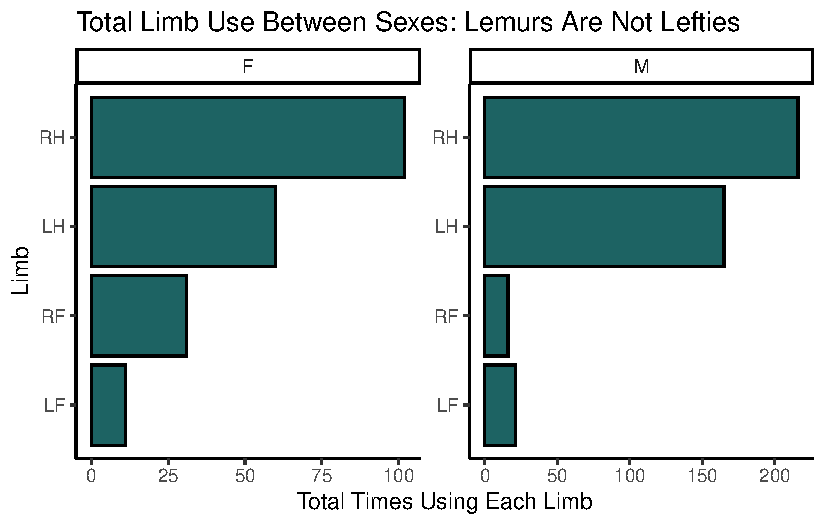
\includegraphics{LeftyLemurs_files/figure-pdf/unnamed-chunk-20-1.pdf}

}

\end{figure}

This is the same thing but just divided by left and right side (left
hand and left foot, etc. are in the same category)

\begin{Shaded}
\begin{Highlighting}[]
\FunctionTok{ggplot}\NormalTok{ (L, }\FunctionTok{aes}\NormalTok{(}\AttributeTok{x=} \FunctionTok{reorder}\NormalTok{ (Side, Side, table ))) }\SpecialCharTok{+}
  \FunctionTok{geom\_bar}\NormalTok{(}\AttributeTok{color =} \StringTok{"black"}\NormalTok{, }\AttributeTok{fill =} \StringTok{"\#1D6363"}\NormalTok{) }\SpecialCharTok{+}
  \FunctionTok{theme\_classic}\NormalTok{() }\SpecialCharTok{+}
  \FunctionTok{xlab}\NormalTok{(}\StringTok{"Left or Right"}\NormalTok{) }\SpecialCharTok{+}
  \FunctionTok{ylab}\NormalTok{(}\StringTok{"Total Times Using Each Limb"}\NormalTok{) }\SpecialCharTok{+}
  \FunctionTok{ggtitle}\NormalTok{(}\StringTok{"Total Limb Use Between Sexes: Lemurs Are Not Lefties"}\NormalTok{) }\SpecialCharTok{+}
  \FunctionTok{coord\_flip}\NormalTok{() }\SpecialCharTok{+}
  \FunctionTok{facet\_wrap}\NormalTok{ (}\SpecialCharTok{\textasciitilde{}}\NormalTok{ Sex, }\AttributeTok{scales =} \StringTok{"free"}\NormalTok{)}
\end{Highlighting}
\end{Shaded}

\begin{figure}[H]

{\centering 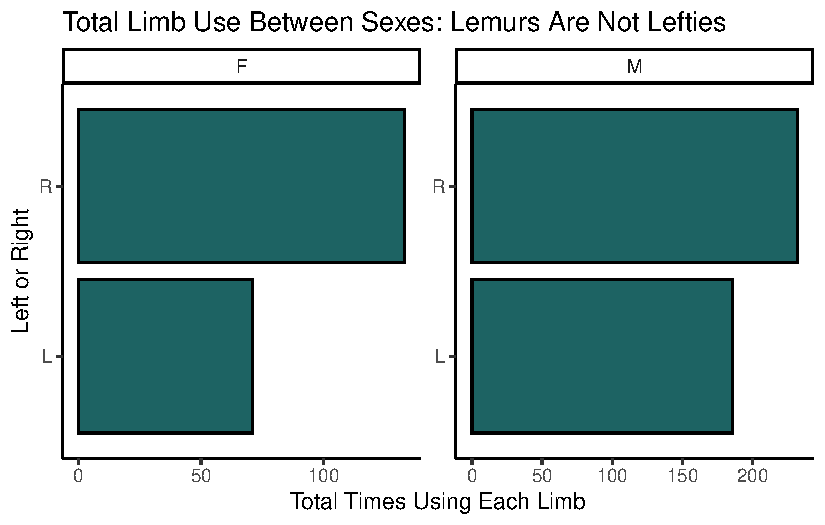
\includegraphics{LeftyLemurs_files/figure-pdf/unnamed-chunk-21-1.pdf}

}

\end{figure}

Definitely more right hand than left HAND use for both males and
females. Not sure about foot use, but I didn't get much foot use data to
begin with. Is there a way to exclude foot use?

Males might me a little less lateralized than females? Left hand use is
also (slightly) higher in males like I thought it would be!

\begin{center}\rule{0.5\linewidth}{0.5pt}\end{center}

\begin{Shaded}
\begin{Highlighting}[]
\FunctionTok{ggplot}\NormalTok{ (L, }\FunctionTok{aes}\NormalTok{(}\AttributeTok{x=} \FunctionTok{reorder}\NormalTok{ (Category, Category, table ))) }\SpecialCharTok{+}
  \FunctionTok{geom\_bar}\NormalTok{(}\AttributeTok{color =} \StringTok{"black"}\NormalTok{, }\AttributeTok{fill =} \StringTok{"\#0577B1"}\NormalTok{) }\SpecialCharTok{+}
  \FunctionTok{theme\_classic}\NormalTok{() }\SpecialCharTok{+}
  \FunctionTok{xlab}\NormalTok{(}\StringTok{"Type of Behavior"}\NormalTok{) }\SpecialCharTok{+}
  \FunctionTok{ylab}\NormalTok{(}\StringTok{"Total Times Using Each Limb"}\NormalTok{) }\SpecialCharTok{+}
  \FunctionTok{ggtitle}\NormalTok{(}\StringTok{"Behavior Across Sexes"}\NormalTok{) }\SpecialCharTok{+}
  \FunctionTok{coord\_flip}\NormalTok{() }\SpecialCharTok{+}
  \FunctionTok{facet\_wrap}\NormalTok{ (}\SpecialCharTok{\textasciitilde{}}\NormalTok{ Sex,}\AttributeTok{scales =} \StringTok{"free"}\NormalTok{)}
\end{Highlighting}
\end{Shaded}

\begin{figure}[H]

{\centering 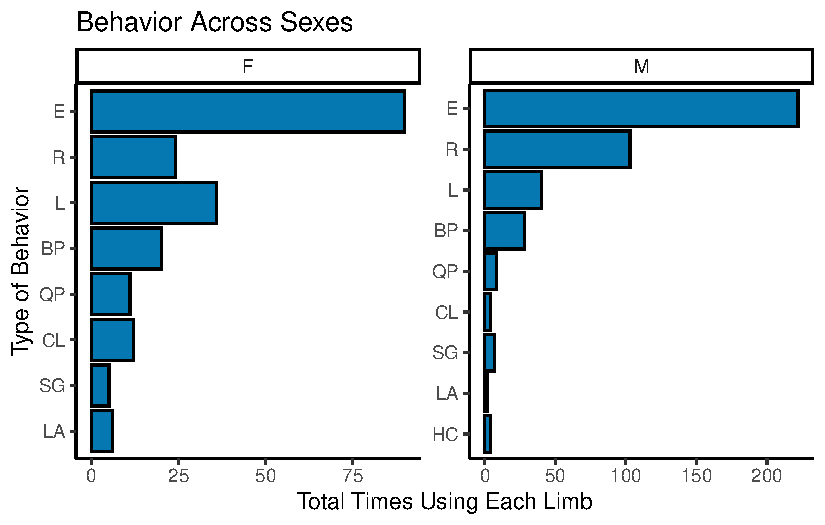
\includegraphics{LeftyLemurs_files/figure-pdf/unnamed-chunk-22-1.pdf}

}

\end{figure}

Everyone eats a lot

Some calculations

\begin{Shaded}
\begin{Highlighting}[]
\FunctionTok{summary}\NormalTok{(L)}
\end{Highlighting}
\end{Shaded}

\begin{verbatim}
    Troop              Focal             Species               Age    
 Length:622         Length:622         Length:622         Min.   : 5  
 Class :character   Class :character   Class :character   1st Qu.:10  
 Mode  :character   Mode  :character   Mode  :character   Median :12  
                                                          Mean   :12  
                                                          3rd Qu.:14  
                                                          Max.   :29  
     Sex                Month            Day             Year     
 Length:622         Min.   :6.000   Min.   : 1.00   Min.   :2022  
 Class :character   1st Qu.:6.000   1st Qu.: 8.00   1st Qu.:2022  
 Mode  :character   Median :6.000   Median :22.00   Median :2022  
                    Mean   :6.436   Mean   :18.04   Mean   :2022  
                    3rd Qu.:7.000   3rd Qu.:28.00   3rd Qu.:2022  
                    Max.   :7.000   Max.   :30.00   Max.   :2022  
     Time             Category             Limb               H.F           
 Length:622         Length:622         Length:622         Length:622        
 Class :character   Class :character   Class :character   Class :character  
 Mode  :character   Mode  :character   Mode  :character   Mode  :character  
                                                                            
                                                                            
                                                                            
     Side               Note          
 Length:622         Length:622        
 Class :character   Class :character  
 Mode  :character   Mode  :character  
                                      
                                      
                                      
\end{verbatim}

\begin{Shaded}
\begin{Highlighting}[]
\FunctionTok{library}\NormalTok{(psych)}
\end{Highlighting}
\end{Shaded}

\begin{verbatim}

Attaching package: 'psych'
\end{verbatim}

\begin{verbatim}
The following objects are masked from 'package:ggplot2':

    %+%, alpha
\end{verbatim}

\begin{Shaded}
\begin{Highlighting}[]
\FunctionTok{describeBy}\NormalTok{(L[}\FunctionTok{c}\NormalTok{(}\DecValTok{4}\NormalTok{,}\DecValTok{1}\SpecialCharTok{:}\DecValTok{12}\NormalTok{)], }\AttributeTok{group =} \StringTok{"Category"}\NormalTok{)}
\end{Highlighting}
\end{Shaded}

\begin{verbatim}

 Descriptive statistics by group 
Category: BP
          vars  n    mean    sd median trimmed   mad  min  max range  skew
Age          1 48    8.71  4.93   10.0    8.00  0.00    5   29    24  2.74
Troop*       2 48    1.17  0.48    1.0    1.05  0.00    1    3     2  2.78
Focal*       3 48    2.54  1.43    2.5    2.55  2.22    1    4     3 -0.04
Species*     4 48    1.96  0.20    2.0    2.00  0.00    1    2     1 -4.44
Age.1        5 48    8.71  4.93   10.0    8.00  0.00    5   29    24  2.74
Sex*         6 48    1.58  0.50    2.0    1.60  0.00    1    2     1 -0.33
Month        7 48    6.56  0.50    7.0    6.58  0.00    6    7     1 -0.24
Day          8 48   12.92 10.58   14.0   12.85 14.83    1   27    26  0.01
Year         9 48 2022.00  0.00 2022.0 2022.00  0.00 2022 2022     0   NaN
Time*       10 48   24.50 14.00   24.5   24.50 17.79    1   48    47  0.00
Category*   11 48    1.00  0.00    1.0    1.00  0.00    1    1     0   NaN
Limb*       12 48    1.56  0.50    2.0    1.57  0.00    1    2     1 -0.24
H.F*        13 48    1.00  0.00    1.0    1.00  0.00    1    1     0   NaN
          kurtosis   se
Age           9.10 0.71
Troop*        6.93 0.07
Focal*       -1.93 0.21
Species*     18.13 0.03
Age.1         9.10 0.71
Sex*         -1.93 0.07
Month        -1.98 0.07
Day          -1.86 1.53
Year           NaN 0.00
Time*        -1.28 2.02
Category*      NaN 0.00
Limb*        -1.98 0.07
H.F*           NaN 0.00
------------------------------------------------------------ 
Category: CL
          vars  n    mean   sd median trimmed  mad  min  max range  skew
Age          1 16   15.25 3.61   17.0   15.86 0.00    5   17    12 -1.74
Troop*       2 16    1.81 0.40    2.0    1.86 0.00    1    2     1 -1.45
Focal*       3 16    2.88 0.72    3.0    2.93 0.00    1    4     3 -0.85
Species*     4 16    1.19 0.40    1.0    1.14 0.00    1    2     1  1.45
Age.1        5 16   15.25 3.61   17.0   15.86 0.00    5   17    12 -1.74
Sex*         6 16    1.25 0.45    1.0    1.21 0.00    1    2     1  1.05
Month        7 16    6.25 0.45    6.0    6.21 0.00    6    7     1  1.05
Day          8 16   18.81 9.52   21.0   19.29 6.67    1   30    29 -0.76
Year         9 16 2022.00 0.00 2022.0 2022.00 0.00 2022 2022     0   NaN
Time*       10 16    8.50 4.76    8.5    8.50 5.93    1   16    15  0.00
Category*   11 16    1.00 0.00    1.0    1.00 0.00    1    1     0   NaN
Limb*       12 16    1.94 0.25    2.0    2.00 0.00    1    2     1 -3.28
H.F*        13 16    1.00 0.00    1.0    1.00 0.00    1    1     0   NaN
          kurtosis   se
Age           1.68 0.90
Troop*        0.13 0.10
Focal*        0.92 0.18
Species*      0.13 0.10
Age.1         1.68 0.90
Sex*         -0.95 0.11
Month        -0.95 0.11
Day          -0.85 2.38
Year           NaN 0.00
Time*        -1.43 1.19
Category*      NaN 0.00
Limb*         9.36 0.06
H.F*           NaN 0.00
------------------------------------------------------------ 
Category: E
          vars   n    mean    sd median trimmed    mad  min  max range   skew
Age          1 312   12.27  7.01   12.0   11.10   2.97    5   29    24   1.23
Troop*       2 312    3.87  1.75    4.0    3.96   1.48    1    6     5  -0.57
Focal*       3 312    7.41  3.47    8.0    7.62   4.45    1   12    11  -0.43
Species*     4 312    1.88  0.85    2.0    1.85   1.48    1    3     2   0.23
Age.1        5 312   12.27  7.01   12.0   11.10   2.97    5   29    24   1.23
Sex*         6 312    1.71  0.45    2.0    1.76   0.00    1    2     1  -0.93
Month        7 312    6.36  0.48    6.0    6.33   0.00    6    7     1   0.57
Day          8 312   19.35 10.46   24.0   20.17   8.90    1   30    29  -0.52
Year         9 312 2022.00  0.00 2022.0 2022.00   0.00 2022 2022     0    NaN
Time*       10 312  154.60 89.04  153.5  154.50 113.42    1  309   308   0.01
Category*   11 312    1.00  0.00    1.0    1.00   0.00    1    1     0    NaN
Limb*       12 312    2.60  0.50    3.0    2.63   0.00    1    3     2  -0.54
H.F*        13 312    1.99  0.08    2.0    2.00   0.00    1    2     1 -12.31
          kurtosis   se
Age           0.98 0.40
Troop*       -1.07 0.10
Focal*       -0.88 0.20
Species*     -1.57 0.05
Age.1         0.98 0.40
Sex*         -1.14 0.03
Month        -1.68 0.03
Day          -1.36 0.59
Year           NaN 0.00
Time*        -1.20 5.04
Category*      NaN 0.00
Limb*        -1.35 0.03
H.F*        150.02 0.00
------------------------------------------------------------ 
Category: HC
          vars n    mean   sd median trimmed  mad  min  max range  skew
Age          1 4   11.50 3.00   10.0   11.50 0.00   10   16     6  0.75
Troop*       2 4    1.25 0.50    1.0    1.25 0.00    1    2     1  0.75
Focal*       3 4    1.75 0.50    2.0    1.75 0.00    1    2     1 -0.75
Species*     4 4    1.75 0.50    2.0    1.75 0.00    1    2     1 -0.75
Age.1        5 4   11.50 3.00   10.0   11.50 0.00   10   16     6  0.75
Sex*         6 4    1.00 0.00    1.0    1.00 0.00    1    1     0   NaN
Month        7 4    6.75 0.50    7.0    6.75 0.00    6    7     1 -0.75
Day          8 4   10.25 8.50    6.0   10.25 0.00    6   23    17  0.75
Year         9 4 2022.00 0.00 2022.0 2022.00 0.00 2022 2022     0   NaN
Time*       10 4    2.50 1.29    2.5    2.50 1.48    1    4     3  0.00
Category*   11 4    1.00 0.00    1.0    1.00 0.00    1    1     0   NaN
Limb*       12 4    1.25 0.50    1.0    1.25 0.00    1    2     1  0.75
H.F*        13 4    1.00 0.00    1.0    1.00 0.00    1    1     0   NaN
          kurtosis   se
Age          -1.69 1.50
Troop*       -1.69 0.25
Focal*       -1.69 0.25
Species*     -1.69 0.25
Age.1        -1.69 1.50
Sex*           NaN 0.00
Month        -1.69 0.25
Day          -1.69 4.25
Year           NaN 0.00
Time*        -2.08 0.65
Category*      NaN 0.00
Limb*        -1.69 0.25
H.F*           NaN 0.00
------------------------------------------------------------ 
Category: L
          vars  n    mean    sd median trimmed   mad  min  max range  skew
Age          1 76   11.78  6.11   12.0   10.98  5.93    5   29    24  1.15
Troop*       2 76    4.12  1.42    5.0    4.24  1.48    1    6     5 -0.84
Focal*       3 76    5.14  3.36    5.0    4.97  4.45    1   12    11  0.15
Species*     4 76    1.59  0.82    1.0    1.50  0.00    1    3     2  0.86
Age.1        5 76   11.78  6.11   12.0   10.98  5.93    5   29    24  1.15
Sex*         6 76    1.53  0.50    2.0    1.53  0.00    1    2     1 -0.10
Month        7 76    6.17  0.38    6.0    6.10  0.00    6    7     1  1.71
Day          8 76   23.16  6.95   27.0   23.98  4.45    6   30    24 -0.91
Year         9 76 2022.00  0.00 2022.0 2022.00  0.00 2022 2022     0   NaN
Time*       10 76   38.49 22.06   38.5   38.50 28.17    1   75    74  0.00
Category*   11 76    1.00  0.00    1.0    1.00  0.00    1    1     0   NaN
Limb*       12 76    2.51  0.53    3.0    2.53  0.00    1    3     2 -0.32
H.F*        13 76    1.99  0.11    2.0    2.00  0.00    1    2     1 -8.38
          kurtosis   se
Age           1.64 0.70
Troop*       -0.39 0.16
Focal*       -1.32 0.39
Species*     -0.99 0.09
Age.1         1.64 0.70
Sex*         -2.02 0.06
Month         0.95 0.04
Day          -0.44 0.80
Year           NaN 0.00
Time*        -1.25 2.53
Category*      NaN 0.00
Limb*        -1.33 0.06
H.F*         69.08 0.01
------------------------------------------------------------ 
Category: LA
          vars n    mean   sd median trimmed  mad  min  max range  skew
Age          1 8   15.12 2.23   16.0   15.12 0.00   10   17     7 -1.42
Troop*       2 8    2.62 0.92    3.0    2.62 0.74    1    4     3 -0.32
Focal*       3 8    2.25 1.58    1.5    2.25 0.74    1    5     4  0.59
Species*     4 8    1.62 0.74    1.5    1.62 0.74    1    3     2  0.54
Age.1        5 8   15.12 2.23   16.0   15.12 0.00   10   17     7 -1.42
Sex*         6 8    1.25 0.46    1.0    1.25 0.00    1    2     1  0.95
Month        7 8    6.62 0.52    7.0    6.62 0.00    6    7     1 -0.42
Day          8 8   14.25 9.33    8.0   14.25 1.48    6   27    21  0.47
Year         9 8 2022.00 0.00 2022.0 2022.00 0.00 2022 2022     0   NaN
Time*       10 8    4.50 2.45    4.5    4.50 2.97    1    8     7  0.00
Category*   11 8    1.00 0.00    1.0    1.00 0.00    1    1     0   NaN
Limb*       12 8    1.62 0.74    1.5    1.62 0.74    1    3     2  0.54
H.F*        13 8    1.50 0.53    1.5    1.50 0.74    1    2     1  0.00
          kurtosis   se
Age           0.56 0.79
Troop*       -1.06 0.32
Focal*       -1.47 0.56
Species*     -1.27 0.26
Age.1         0.56 0.79
Sex*         -1.21 0.16
Month        -2.03 0.18
Day          -1.89 3.30
Year           NaN 0.00
Time*        -1.65 0.87
Category*      NaN 0.00
Limb*        -1.27 0.26
H.F*         -2.23 0.19
------------------------------------------------------------ 
Category: QP
          vars  n    mean   sd median trimmed  mad  min  max range  skew
Age          1 19   16.37 3.30     16   15.76 1.48   14   29    15  2.83
Troop*       2 19    1.68 0.75      2    1.65 1.48    1    3     2  0.52
Focal*       3 19    3.84 1.95      4    3.88 2.97    1    6     5 -0.26
Species*     4 19    1.63 0.50      2    1.65 0.00    1    2     1 -0.50
Age.1        5 19   16.37 3.30     16   15.76 1.48   14   29    15  2.83
Sex*         6 19    1.42 0.51      1    1.41 0.00    1    2     1  0.29
Month        7 19    6.11 0.32      6    6.06 0.00    6    7     1  2.37
Day          8 19   23.89 6.53     27   24.71 2.97    5   29    24 -1.93
Year         9 19 2022.00 0.00   2022 2022.00 0.00 2022 2022     0   NaN
Time*       10 19   10.00 5.63     10   10.00 7.41    1   19    18  0.00
Category*   11 19    1.00 0.00      1    1.00 0.00    1    1     0   NaN
Limb*       12 19    2.47 0.77      3    2.53 0.00    1    3     2 -0.95
H.F*        13 19    1.84 0.37      2    1.88 0.00    1    2     1 -1.73
          kurtosis   se
Age           8.34 0.76
Troop*       -1.16 0.17
Focal*       -1.52 0.45
Species*     -1.84 0.11
Age.1         8.34 0.76
Sex*         -2.01 0.12
Month         3.84 0.07
Day           2.60 1.50
Year           NaN 0.00
Time*        -1.39 1.29
Category*      NaN 0.00
Limb*        -0.74 0.18
H.F*          1.06 0.09
------------------------------------------------------------ 
Category: R
          vars   n    mean    sd median trimmed   mad  min  max range   skew
Age          1 127   11.50  5.25     10   10.72  2.97    5   29    24   2.09
Troop*       2 127    2.70  1.16      3    2.65  0.00    1    5     4  -0.05
Focal*       3 127    5.31  2.48      6    5.31  4.45    1    9     8   0.00
Species*     4 127    2.67  0.69      3    2.83  0.00    1    3     2  -1.76
Age.1        5 127   11.50  5.25     10   10.72  2.97    5   29    24   2.09
Sex*         6 127    1.81  0.39      2    1.88  0.00    1    2     1  -1.57
Month        7 127    6.81  0.39      7    6.88  0.00    6    7     1  -1.57
Day          8 127   12.51  8.69     12   11.87  5.93    1   30    29   0.63
Year         9 127 2022.00  0.00   2022 2022.00  0.00 2022 2022     0    NaN
Time*       10 127   64.00 36.81     64   64.00 47.44    1  127   126   0.00
Category*   11 127    1.00  0.00      1    1.00  0.00    1    1     0    NaN
Limb*       12 127    2.17  0.98      3    2.21  0.00    1    3     2  -0.35
H.F*        13 127    1.99  0.09      2    2.00  0.00    1    2     1 -11.00
          kurtosis   se
Age           5.16 0.47
Troop*       -0.50 0.10
Focal*       -1.40 0.22
Species*      1.41 0.06
Age.1         5.16 0.47
Sex*          0.47 0.03
Month         0.47 0.03
Day          -0.37 0.77
Year           NaN 0.00
Time*        -1.23 3.27
Category*      NaN 0.00
Limb*        -1.89 0.09
H.F*        120.05 0.01
------------------------------------------------------------ 
Category: SG
          vars  n    mean   sd median trimmed  mad  min  max range  skew
Age          1 12   11.67 5.21   15.0    11.9 1.48    5   16    11 -0.41
Troop*       2 12    2.00 0.95    2.0     1.9 1.48    1    4     3  0.58
Focal*       3 12    3.42 1.56    3.5     3.5 2.22    1    5     4 -0.12
Species*     4 12    2.25 0.75    2.0     2.3 1.48    1    3     2 -0.36
Age.1        5 12   11.67 5.21   15.0    11.9 1.48    5   16    11 -0.41
Sex*         6 12    1.58 0.51    2.0     1.6 0.00    1    2     1 -0.30
Month        7 12    6.08 0.29    6.0     6.0 0.00    6    7     1  2.65
Day          8 12   25.25 3.93   27.0    26.0 0.00   14   29    15 -1.85
Year         9 12 2022.00 0.00 2022.0  2022.0 0.00 2022 2022     0   NaN
Time*       10 12    6.50 3.61    6.5     6.5 4.45    1   12    11  0.00
Category*   11 12    1.00 0.00    1.0     1.0 0.00    1    1     0   NaN
Limb*       12 12    1.67 0.78    1.5     1.6 0.74    1    3     2  0.55
H.F*        13 12    1.67 0.49    2.0     1.7 0.00    1    2     1 -0.62
          kurtosis   se
Age          -1.86 1.50
Troop*       -0.78 0.28
Focal*       -1.86 0.45
Species*     -1.33 0.22
Age.1        -1.86 1.50
Sex*         -2.06 0.15
Month         5.48 0.08
Day           2.67 1.14
Year           NaN 0.00
Time*        -1.50 1.04
Category*      NaN 0.00
Limb*        -1.29 0.22
H.F*         -1.74 0.14
\end{verbatim}

\begin{Shaded}
\begin{Highlighting}[]
\CommentTok{\# what does the 4 mean??}
\end{Highlighting}
\end{Shaded}

Making a DF with just hand grasp data

\begin{Shaded}
\begin{Highlighting}[]
\CommentTok{\# take out feet use data}

\NormalTok{l\_hands }\OtherTok{\textless{}{-}}
\NormalTok{  L }\SpecialCharTok{\%\textgreater{}\%}
  \FunctionTok{select}\NormalTok{(H.F) }\SpecialCharTok{\%\textgreater{}\%}
  \FunctionTok{filter}\NormalTok{(}\FunctionTok{str\_detect}\NormalTok{(H.F, }\StringTok{"H"}\NormalTok{))}

\CommentTok{\# add the other stuff back}
\NormalTok{l\_hands }\OtherTok{\textless{}{-}} \FunctionTok{inner\_join}\NormalTok{(l\_hands, L, }\AttributeTok{by =} \StringTok{"H.F"}\NormalTok{)}

\NormalTok{l\_hands }\OtherTok{\textless{}{-}} \FunctionTok{unique}\NormalTok{(l\_hands)}

\CommentTok{\# actually I also don\textquotesingle{}t want to look at all the categories bc some were added just for fun and are probably not important}

\NormalTok{l\_handstuff }\OtherTok{\textless{}{-}}
\NormalTok{  l\_hands }\SpecialCharTok{\%\textgreater{}\%}
  \FunctionTok{select}\NormalTok{(Category) }\SpecialCharTok{\%\textgreater{}\%}
  \FunctionTok{filter}\NormalTok{(}\FunctionTok{str\_detect}\NormalTok{(Category, }\StringTok{"E|L|R|SG"}\NormalTok{))}


\CommentTok{\# WHY WON\textquotesingle{}T IT TAKE OUT LA}

\CommentTok{\# add the other stuff back why did it even go away}

\NormalTok{l\_handstuff }\OtherTok{\textless{}{-}} \FunctionTok{inner\_join}\NormalTok{(l\_handstuff, l\_hands, }\AttributeTok{by =} \StringTok{"Category"}\NormalTok{)}

\CommentTok{\# I can remove the H.F row because all of it is hand }

\NormalTok{l\_handstuff }\OtherTok{\textless{}{-}}\NormalTok{ l\_handstuff }\SpecialCharTok{\%\textgreater{}\%} \FunctionTok{select}\NormalTok{(}\SpecialCharTok{{-}}\NormalTok{H.F)}

\CommentTok{\# removing Limb row bc side says the same thing}

\NormalTok{l\_handstuff }\OtherTok{\textless{}{-}}\NormalTok{ l\_handstuff }\SpecialCharTok{\%\textgreater{}\%} \FunctionTok{select}\NormalTok{(}\SpecialCharTok{{-}}\NormalTok{Limb)}

\CommentTok{\# removing mystery duplicates}

\NormalTok{l\_handstuff }\OtherTok{\textless{}{-}} \FunctionTok{unique}\NormalTok{(l\_handstuff)}


\NormalTok{l\_noLA }\OtherTok{\textless{}{-}} 
\NormalTok{l\_handstuff }\SpecialCharTok{\%\textgreater{}\%} 
  \FunctionTok{filter}\NormalTok{(Category }\SpecialCharTok{==} \StringTok{"E"}  \SpecialCharTok{|}\NormalTok{  Category }\SpecialCharTok{==} \StringTok{"L"} \SpecialCharTok{|}\NormalTok{  Category }\SpecialCharTok{==} \StringTok{"R"} \SpecialCharTok{|}\NormalTok{  Category }\SpecialCharTok{==} \StringTok{"SG"} \SpecialCharTok{|}\NormalTok{ Category }\SpecialCharTok{!=} \StringTok{"LA"}\NormalTok{ )}

\CommentTok{\#wow I forgot you can do that}
\end{Highlighting}
\end{Shaded}

Compare hand use by species

\begin{Shaded}
\begin{Highlighting}[]
\FunctionTok{ggplot}\NormalTok{ (l\_noLA, }\FunctionTok{aes}\NormalTok{(}\AttributeTok{x=}\NormalTok{ Side)) }\SpecialCharTok{+}
  \FunctionTok{geom\_bar}\NormalTok{(}\AttributeTok{color =} \StringTok{"black"}\NormalTok{, }\AttributeTok{fill =} \StringTok{"\#C84E00"}\NormalTok{) }\SpecialCharTok{+}
  \FunctionTok{theme\_classic}\NormalTok{() }\SpecialCharTok{+}
  \FunctionTok{xlab}\NormalTok{(}\StringTok{"Left or Right Side"}\NormalTok{) }\SpecialCharTok{+}
  \FunctionTok{ylab}\NormalTok{(}\StringTok{"\# of Times Using Each Limb"}\NormalTok{) }\SpecialCharTok{+}
  \FunctionTok{ggtitle}\NormalTok{(}\StringTok{"Hand Use Between Lemur Species"}\NormalTok{) }\SpecialCharTok{+}
  \FunctionTok{facet\_wrap}\NormalTok{ (}\SpecialCharTok{\textasciitilde{}}\NormalTok{ Species, }\AttributeTok{scales =} \StringTok{"free"}\NormalTok{)}
\end{Highlighting}
\end{Shaded}

\begin{figure}[H]

{\centering 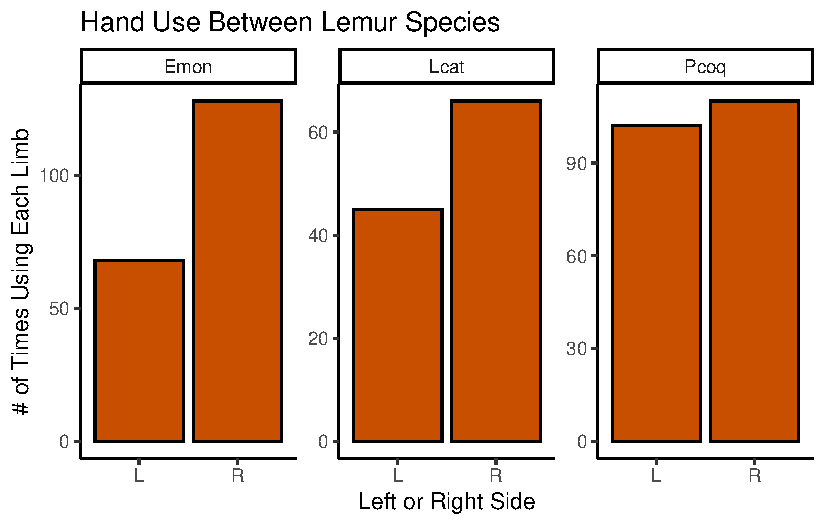
\includegraphics{LeftyLemurs_files/figure-pdf/unnamed-chunk-25-1.pdf}

}

\end{figure}

\begin{Shaded}
\begin{Highlighting}[]
\FunctionTok{ggplot}\NormalTok{ (l\_noLA, }\FunctionTok{aes}\NormalTok{(}\AttributeTok{x=}\NormalTok{ Side)) }\SpecialCharTok{+}
  \FunctionTok{geom\_bar}\NormalTok{(}\AttributeTok{color =} \StringTok{"black"}\NormalTok{, }\AttributeTok{fill =} \StringTok{"\#C84E00"}\NormalTok{) }\SpecialCharTok{+}
  \FunctionTok{theme\_classic}\NormalTok{() }\SpecialCharTok{+}
  \FunctionTok{xlab}\NormalTok{(}\StringTok{"Left or Right Side"}\NormalTok{) }\SpecialCharTok{+}
  \FunctionTok{ylab}\NormalTok{(}\StringTok{"Type of Behavior"}\NormalTok{) }\SpecialCharTok{+}
  \FunctionTok{ggtitle}\NormalTok{(}\StringTok{"Hand Use Between Behaviors"}\NormalTok{) }\SpecialCharTok{+}
  \FunctionTok{facet\_wrap}\NormalTok{ (}\SpecialCharTok{\textasciitilde{}}\NormalTok{ Category, }\AttributeTok{scales =} \StringTok{"free"}\NormalTok{)}
\end{Highlighting}
\end{Shaded}

\begin{figure}[H]

{\centering 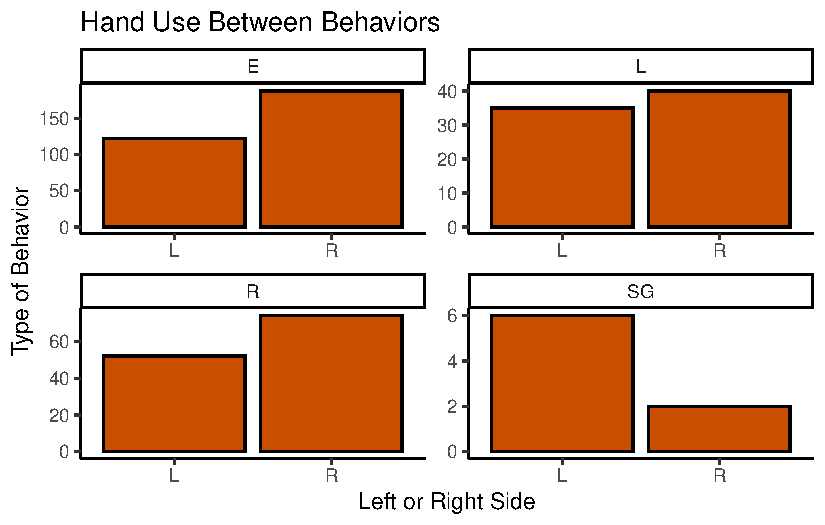
\includegraphics{LeftyLemurs_files/figure-pdf/unnamed-chunk-26-1.pdf}

}

\end{figure}

So it looks like lemurs mostly use their right hand for everything
except for grooming! Interesting

Now I'm going to filter out the grooming data so it's all grasping

\begin{Shaded}
\begin{Highlighting}[]
\NormalTok{l\_grasps }\OtherTok{\textless{}{-}}
\NormalTok{l\_noLA }\SpecialCharTok{\%\textgreater{}\%} 
  \FunctionTok{filter}\NormalTok{(Category }\SpecialCharTok{==} \StringTok{"E"}  \SpecialCharTok{|}\NormalTok{  Category }\SpecialCharTok{==} \StringTok{"L"} \SpecialCharTok{|}\NormalTok{  Category }\SpecialCharTok{==} \StringTok{"R"}\NormalTok{)}
\end{Highlighting}
\end{Shaded}

Compare grasping hand by species

\begin{Shaded}
\begin{Highlighting}[]
\FunctionTok{ggplot}\NormalTok{ (l\_grasps, }\FunctionTok{aes}\NormalTok{(}\AttributeTok{x=}\NormalTok{ Side)) }\SpecialCharTok{+}
  \FunctionTok{geom\_bar}\NormalTok{(}\AttributeTok{color =} \StringTok{"black"}\NormalTok{, }\AttributeTok{fill =} \StringTok{"\#C84E00"}\NormalTok{) }\SpecialCharTok{+}
  \FunctionTok{theme\_classic}\NormalTok{() }\SpecialCharTok{+}
  \FunctionTok{xlab}\NormalTok{(}\StringTok{"Left or Right Side"}\NormalTok{) }\SpecialCharTok{+}
  \FunctionTok{ylab}\NormalTok{(}\StringTok{"\# of Times Using Each Limb"}\NormalTok{) }\SpecialCharTok{+}
  \FunctionTok{ggtitle}\NormalTok{(}\StringTok{"Hand Use for Grasping Between Lemur Species"}\NormalTok{) }\SpecialCharTok{+}
  \FunctionTok{facet\_wrap}\NormalTok{ (}\SpecialCharTok{\textasciitilde{}}\NormalTok{ Species, }\AttributeTok{scales =} \StringTok{"free"}\NormalTok{)}
\end{Highlighting}
\end{Shaded}

\begin{figure}[H]

{\centering 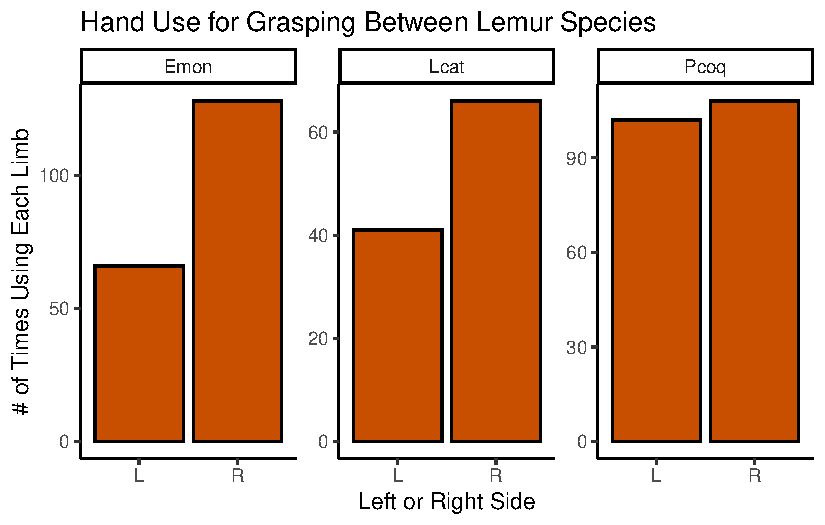
\includegraphics{LeftyLemurs_files/figure-pdf/unnamed-chunk-28-1.pdf}

}

\end{figure}

What about by sex?

\begin{Shaded}
\begin{Highlighting}[]
\FunctionTok{ggplot}\NormalTok{ (l\_grasps, }\FunctionTok{aes}\NormalTok{(}\AttributeTok{x=}\NormalTok{ Side)) }\SpecialCharTok{+}
  \FunctionTok{geom\_bar}\NormalTok{(}\AttributeTok{color =} \StringTok{"black"}\NormalTok{, }\AttributeTok{fill =} \StringTok{"\#C84E00"}\NormalTok{) }\SpecialCharTok{+}
  \FunctionTok{theme\_classic}\NormalTok{() }\SpecialCharTok{+}
  \FunctionTok{xlab}\NormalTok{(}\StringTok{"Left or Right Side"}\NormalTok{) }\SpecialCharTok{+}
  \FunctionTok{ylab}\NormalTok{(}\StringTok{"\# of Times Using Each Limb"}\NormalTok{) }\SpecialCharTok{+}
  \FunctionTok{ggtitle}\NormalTok{(}\StringTok{"Hand Use for Grasping Between Sexes"}\NormalTok{) }\SpecialCharTok{+}
  \FunctionTok{facet\_wrap}\NormalTok{ (}\SpecialCharTok{\textasciitilde{}}\NormalTok{ Sex, }\AttributeTok{scales =} \StringTok{"free"}\NormalTok{)}
\end{Highlighting}
\end{Shaded}

\begin{figure}[H]

{\centering 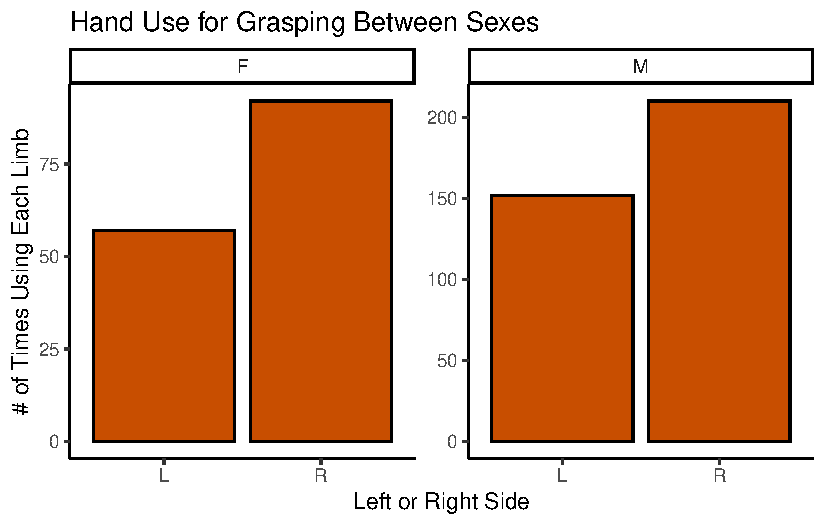
\includegraphics{LeftyLemurs_files/figure-pdf/unnamed-chunk-29-1.pdf}

}

\end{figure}

It doesn't look like there's really a difference

What about just food grasps?

\begin{Shaded}
\begin{Highlighting}[]
\NormalTok{l\_foodGrasps }\OtherTok{\textless{}{-}}
\NormalTok{l\_grasps }\SpecialCharTok{\%\textgreater{}\%} 
  \FunctionTok{filter}\NormalTok{(Category }\SpecialCharTok{==} \StringTok{"E"}\NormalTok{)}
\end{Highlighting}
\end{Shaded}

Compare grasping hand by species

\begin{Shaded}
\begin{Highlighting}[]
\FunctionTok{ggplot}\NormalTok{ (l\_foodGrasps, }\FunctionTok{aes}\NormalTok{(}\AttributeTok{x=}\NormalTok{ Side)) }\SpecialCharTok{+}
  \FunctionTok{geom\_bar}\NormalTok{(}\AttributeTok{color =} \StringTok{"black"}\NormalTok{, }\AttributeTok{fill =} \StringTok{"\#C84E00"}\NormalTok{) }\SpecialCharTok{+}
  \FunctionTok{theme\_classic}\NormalTok{() }\SpecialCharTok{+}
  \FunctionTok{xlab}\NormalTok{(}\StringTok{"Left or Right Side"}\NormalTok{) }\SpecialCharTok{+}
  \FunctionTok{ylab}\NormalTok{(}\StringTok{"\# of Times Using Each Limb"}\NormalTok{) }\SpecialCharTok{+}
  \FunctionTok{ggtitle}\NormalTok{(}\StringTok{"Hand Use for Food Grasping Between Lemur Species"}\NormalTok{) }\SpecialCharTok{+}
  \FunctionTok{facet\_wrap}\NormalTok{ (}\SpecialCharTok{\textasciitilde{}}\NormalTok{ Species, }\AttributeTok{scales =} \StringTok{"free"}\NormalTok{)}
\end{Highlighting}
\end{Shaded}

\begin{figure}[H]

{\centering 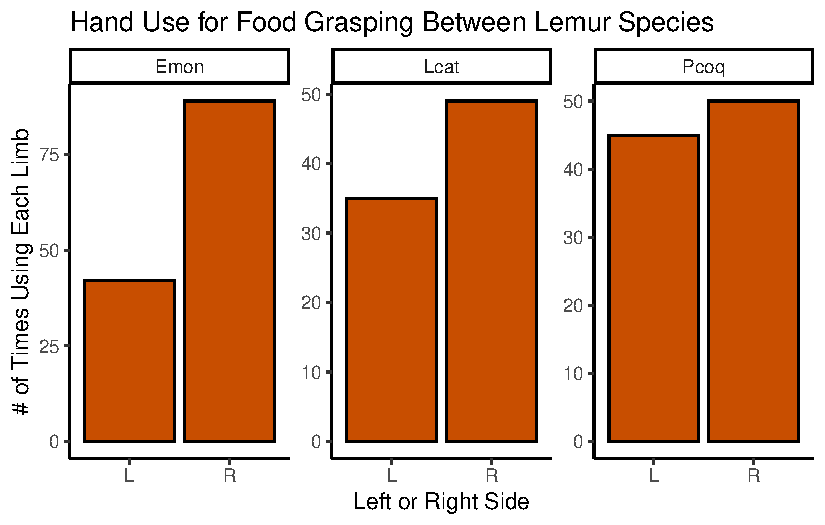
\includegraphics{LeftyLemurs_files/figure-pdf/unnamed-chunk-31-1.pdf}

}

\end{figure}

It really looks like sifakas are more ambidextrous when it comes to food
grasping!

What about by individual?

\begin{Shaded}
\begin{Highlighting}[]
\FunctionTok{ggplot}\NormalTok{ (l\_foodGrasps, }\FunctionTok{aes}\NormalTok{(}\AttributeTok{x=}\NormalTok{ Side)) }\SpecialCharTok{+}
  \FunctionTok{geom\_bar}\NormalTok{(}\AttributeTok{color =} \StringTok{"black"}\NormalTok{, }\AttributeTok{fill =} \StringTok{"\#C84E00"}\NormalTok{) }\SpecialCharTok{+}
  \FunctionTok{theme\_classic}\NormalTok{() }\SpecialCharTok{+}
  \FunctionTok{xlab}\NormalTok{(}\StringTok{"Left or Right Side"}\NormalTok{) }\SpecialCharTok{+}
  \FunctionTok{ylab}\NormalTok{(}\StringTok{"\# of Times Using Each Limb"}\NormalTok{) }\SpecialCharTok{+}
  \FunctionTok{ggtitle}\NormalTok{(}\StringTok{"Hand Use for Food Grasping Between Individuals"}\NormalTok{) }\SpecialCharTok{+}
  \FunctionTok{facet\_wrap}\NormalTok{ (}\SpecialCharTok{\textasciitilde{}}\NormalTok{ Focal, }\AttributeTok{scales =} \StringTok{"free"}\NormalTok{)}
\end{Highlighting}
\end{Shaded}

\begin{figure}[H]

{\centering 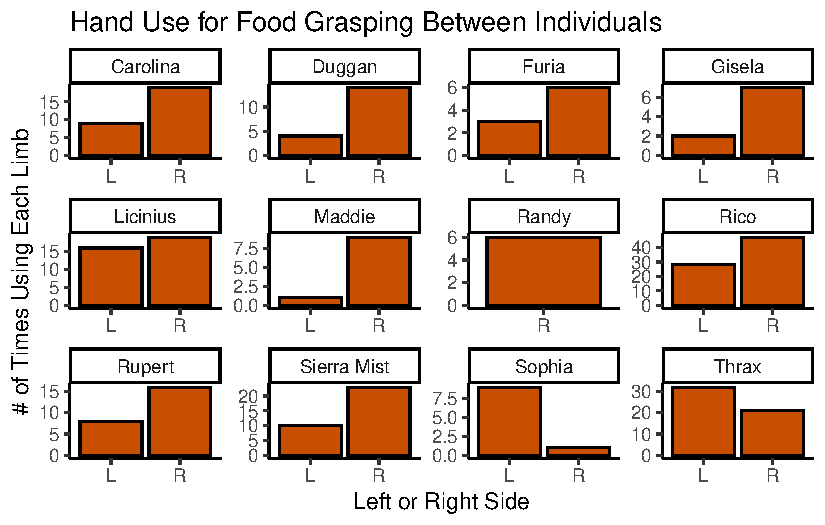
\includegraphics{LeftyLemurs_files/figure-pdf/unnamed-chunk-32-1.pdf}

}

\end{figure}

It kind of looks like Sophia and Thrax are lefties!!! And Licinius is
close\ldots{} The other lemurs look like righties!

Look at them all on the same scale

\begin{Shaded}
\begin{Highlighting}[]
\FunctionTok{ggplot}\NormalTok{ (l\_foodGrasps, }\FunctionTok{aes}\NormalTok{(}\AttributeTok{x=}\NormalTok{ Side)) }\SpecialCharTok{+}
  \FunctionTok{geom\_bar}\NormalTok{(}\AttributeTok{color =} \StringTok{"black"}\NormalTok{, }\AttributeTok{fill =} \StringTok{"\#C84E00"}\NormalTok{) }\SpecialCharTok{+}
  \FunctionTok{theme\_classic}\NormalTok{() }\SpecialCharTok{+}
  \FunctionTok{xlab}\NormalTok{(}\StringTok{"Left or Right Side"}\NormalTok{) }\SpecialCharTok{+}
  \FunctionTok{ylab}\NormalTok{(}\StringTok{"\# of Times Using Each Limb"}\NormalTok{) }\SpecialCharTok{+}
  \FunctionTok{ggtitle}\NormalTok{(}\StringTok{"Hand Use for Food Grasping Between Individuals"}\NormalTok{) }\SpecialCharTok{+}
  \FunctionTok{facet\_wrap}\NormalTok{ (}\SpecialCharTok{\textasciitilde{}}\NormalTok{ Focal)}
\end{Highlighting}
\end{Shaded}

\begin{figure}[H]

{\centering 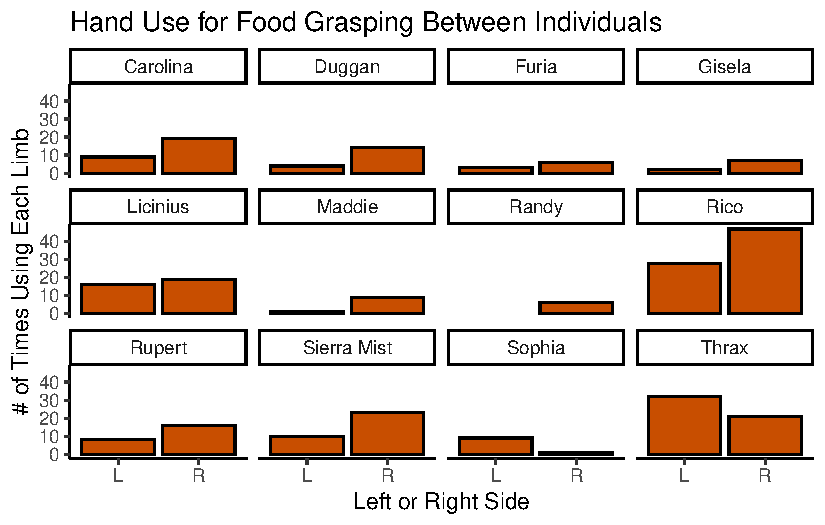
\includegraphics{LeftyLemurs_files/figure-pdf/unnamed-chunk-33-1.pdf}

}

\end{figure}

Okay there isn't much data for Sophia so it could just be ``noise'' for
her\ldots{} But Thrax has a lot of data

But is all of this actually statistically significant Don't know

\begin{Shaded}
\begin{Highlighting}[]
\FunctionTok{ggplot}\NormalTok{ (l\_noLA, }\FunctionTok{aes}\NormalTok{(}\AttributeTok{x=}\NormalTok{ Category)) }\SpecialCharTok{+}
  \FunctionTok{geom\_bar}\NormalTok{(}\AttributeTok{color =} \StringTok{"black"}\NormalTok{, }\AttributeTok{fill =} \StringTok{"\#C84E00"}\NormalTok{) }\SpecialCharTok{+}
  \FunctionTok{theme\_classic}\NormalTok{() }\SpecialCharTok{+}
  \FunctionTok{xlab}\NormalTok{(}\StringTok{"Activity"}\NormalTok{) }\SpecialCharTok{+}
  \FunctionTok{ylab}\NormalTok{(}\StringTok{"Occurrences"}\NormalTok{) }\SpecialCharTok{+}
  \FunctionTok{ggtitle}\NormalTok{(}\StringTok{"Hand Use for Activities by Species"}\NormalTok{) }\SpecialCharTok{+}
  \FunctionTok{facet\_wrap}\NormalTok{ (}\SpecialCharTok{\textasciitilde{}}\NormalTok{ Species)}
\end{Highlighting}
\end{Shaded}

\begin{figure}[H]

{\centering 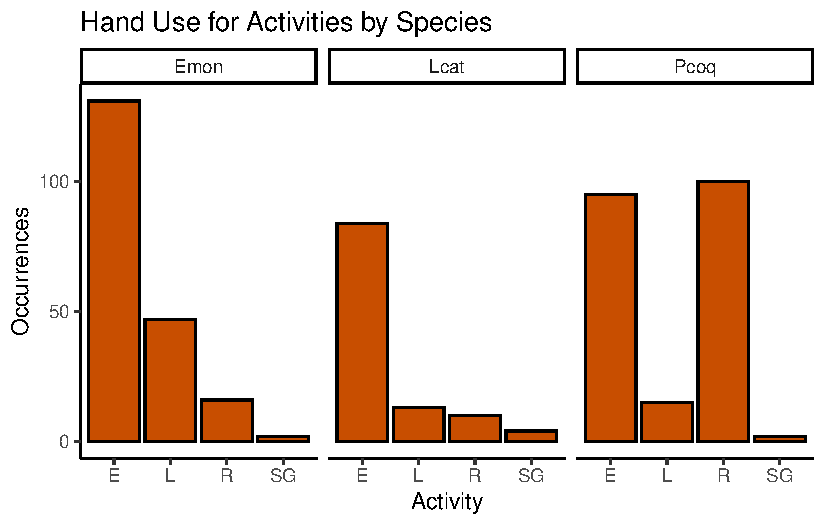
\includegraphics{LeftyLemurs_files/figure-pdf/unnamed-chunk-34-1.pdf}

}

\end{figure}

This just does occurrences. How can I get the Y-axis to be \% of L
compared to R?

Idk

\begin{Shaded}
\begin{Highlighting}[]
\FunctionTok{ggplot}\NormalTok{ (l\_foodGrasps, }\FunctionTok{aes}\NormalTok{(}\AttributeTok{x=}\NormalTok{ Side)) }\SpecialCharTok{+}
  \FunctionTok{geom\_bar}\NormalTok{(}\AttributeTok{color =} \StringTok{"black"}\NormalTok{, }\AttributeTok{fill =} \StringTok{"\#C84E00"}\NormalTok{) }\SpecialCharTok{+}
  \FunctionTok{theme\_classic}\NormalTok{() }\SpecialCharTok{+}
  \FunctionTok{xlab}\NormalTok{(}\StringTok{"Activity"}\NormalTok{) }\SpecialCharTok{+}
  \FunctionTok{ylab}\NormalTok{(}\StringTok{"Occurrences"}\NormalTok{) }\SpecialCharTok{+}
  \FunctionTok{ggtitle}\NormalTok{(}\StringTok{"Hand Used for Food Grasping Between Species"}\NormalTok{) }\SpecialCharTok{+}
  \FunctionTok{facet\_wrap}\NormalTok{ (}\SpecialCharTok{\textasciitilde{}}\NormalTok{ Species)}
\end{Highlighting}
\end{Shaded}

\begin{figure}[H]

{\centering 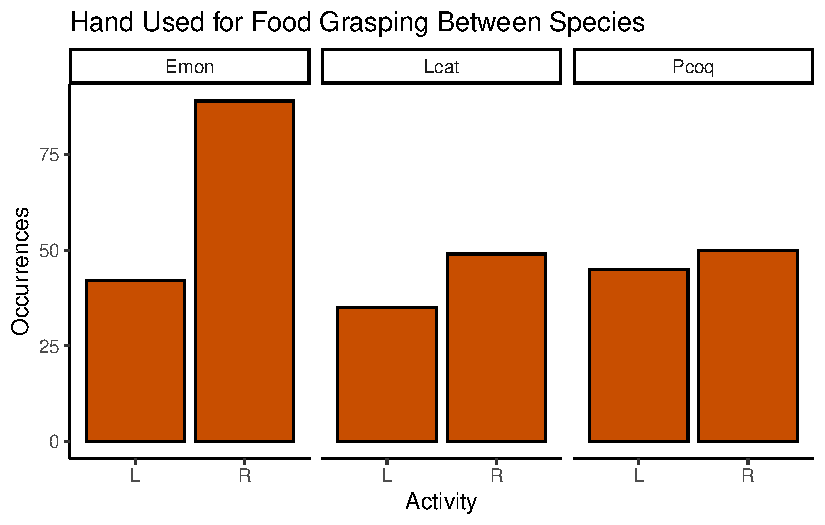
\includegraphics{LeftyLemurs_files/figure-pdf/unnamed-chunk-35-1.pdf}

}

\end{figure}

\begin{Shaded}
\begin{Highlighting}[]
\FunctionTok{ggplot}\NormalTok{ (l\_foodGrasps, }\FunctionTok{aes}\NormalTok{(}\AttributeTok{x=}\NormalTok{ Side)) }\SpecialCharTok{+}
  \FunctionTok{geom\_bar}\NormalTok{(}\AttributeTok{color =} \StringTok{"black"}\NormalTok{, }\AttributeTok{fill =} \StringTok{"\#C84E00"}\NormalTok{) }\SpecialCharTok{+}
  \FunctionTok{theme\_classic}\NormalTok{() }\SpecialCharTok{+}
  \FunctionTok{xlab}\NormalTok{(}\StringTok{"Left or Right Side"}\NormalTok{) }\SpecialCharTok{+}
  \FunctionTok{ylab}\NormalTok{(}\StringTok{"\# of Times Using Each Limb"}\NormalTok{) }\SpecialCharTok{+}
  \FunctionTok{ggtitle}\NormalTok{(}\StringTok{"Hand Use for Grasping Between Individuals"}\NormalTok{) }\SpecialCharTok{+}
  \FunctionTok{facet\_wrap}\NormalTok{ (}\SpecialCharTok{\textasciitilde{}}\NormalTok{ Focal, }\AttributeTok{scales =} \StringTok{"free"}\NormalTok{ )}
\end{Highlighting}
\end{Shaded}

\begin{figure}[H]

{\centering 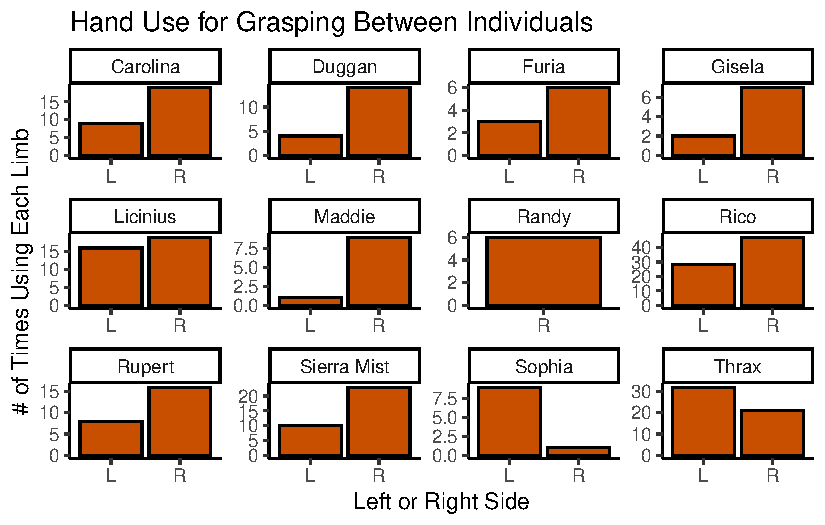
\includegraphics{LeftyLemurs_files/figure-pdf/unnamed-chunk-36-1.pdf}

}

\end{figure}

\begin{Shaded}
\begin{Highlighting}[]
\FunctionTok{ggplot}\NormalTok{ (l\_foodGrasps, }\FunctionTok{aes}\NormalTok{(}\AttributeTok{x=}\NormalTok{ Side)) }\SpecialCharTok{+}
  \FunctionTok{geom\_bar}\NormalTok{(}\AttributeTok{color =} \StringTok{"black"}\NormalTok{, }\AttributeTok{fill =} \StringTok{"\#C84E00"}\NormalTok{) }\SpecialCharTok{+}
  \FunctionTok{theme\_classic}\NormalTok{() }\SpecialCharTok{+}
  \FunctionTok{xlab}\NormalTok{(}\StringTok{"Side"}\NormalTok{) }\SpecialCharTok{+}
  \FunctionTok{ylab}\NormalTok{(}\StringTok{"Occurrences"}\NormalTok{) }\SpecialCharTok{+}
  \FunctionTok{ggtitle}\NormalTok{(}\StringTok{"Hand Used for Food Grasping Between Species"}\NormalTok{) }\SpecialCharTok{+}
  \FunctionTok{facet\_wrap}\NormalTok{ (}\SpecialCharTok{\textasciitilde{}}\NormalTok{ Species)}
\end{Highlighting}
\end{Shaded}

\begin{figure}[H]

{\centering 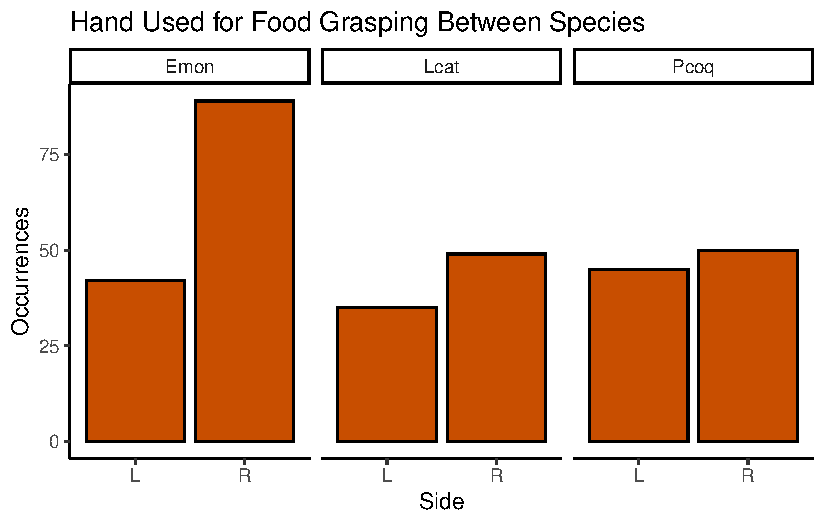
\includegraphics{LeftyLemurs_files/figure-pdf/unnamed-chunk-37-1.pdf}

}

\end{figure}

\begin{Shaded}
\begin{Highlighting}[]
\FunctionTok{ggplot}\NormalTok{ (L, }\FunctionTok{aes}\NormalTok{(}\AttributeTok{x=}\NormalTok{ Focal)) }\SpecialCharTok{+}
  \FunctionTok{geom\_bar}\NormalTok{(}\AttributeTok{color =} \StringTok{"black"}\NormalTok{, }\AttributeTok{fill =} \StringTok{"\#C84E00"}\NormalTok{) }\SpecialCharTok{+}
  \FunctionTok{theme\_classic}\NormalTok{() }\SpecialCharTok{+}
  \FunctionTok{xlab}\NormalTok{(}\StringTok{"Focal"}\NormalTok{) }\SpecialCharTok{+}
  \FunctionTok{ylab}\NormalTok{(}\StringTok{"Occurrences"}\NormalTok{) }\SpecialCharTok{+}
  \FunctionTok{ggtitle}\NormalTok{(}\StringTok{"\# of Times Using Each Limb"}\NormalTok{) }\SpecialCharTok{+}
  \FunctionTok{facet\_wrap}\NormalTok{ (}\SpecialCharTok{\textasciitilde{}}\NormalTok{ Side)}
\end{Highlighting}
\end{Shaded}

\begin{figure}[H]

{\centering 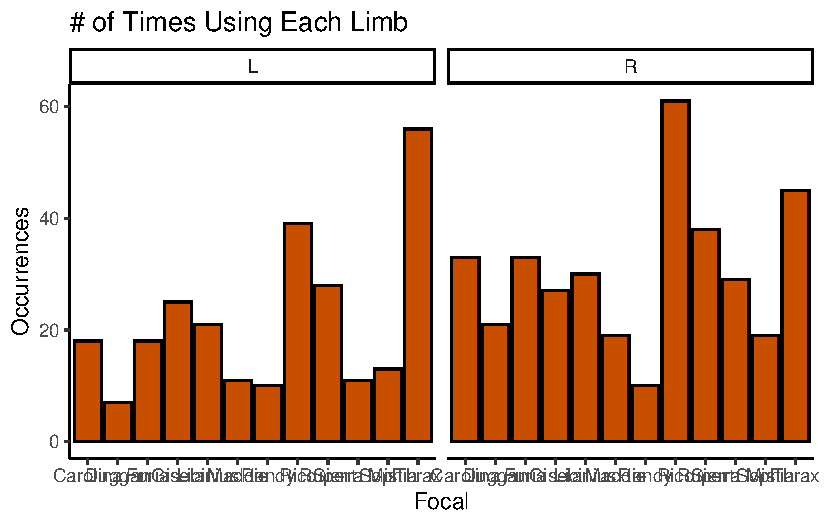
\includegraphics{LeftyLemurs_files/figure-pdf/unnamed-chunk-38-1.pdf}

}

\end{figure}

\begin{Shaded}
\begin{Highlighting}[]
\FunctionTok{ggplot}\NormalTok{ (l\_foodGrasps, }\FunctionTok{aes}\NormalTok{(}\AttributeTok{x=}\NormalTok{ Side)) }\SpecialCharTok{+}
  \FunctionTok{geom\_bar}\NormalTok{(}\AttributeTok{color =} \StringTok{"black"}\NormalTok{, }\AttributeTok{fill =} \StringTok{"\#C84E00"}\NormalTok{) }\SpecialCharTok{+}
  \FunctionTok{theme\_classic}\NormalTok{() }\SpecialCharTok{+}
  \FunctionTok{xlab}\NormalTok{(}\StringTok{"Side"}\NormalTok{) }\SpecialCharTok{+}
  \FunctionTok{ylab}\NormalTok{(}\StringTok{"Occurrences"}\NormalTok{) }\SpecialCharTok{+}
  \FunctionTok{ggtitle}\NormalTok{(}\StringTok{"Hand Used for Food Grasping Between Sex"}\NormalTok{) }\SpecialCharTok{+}
  \FunctionTok{facet\_wrap}\NormalTok{ (}\SpecialCharTok{\textasciitilde{}}\NormalTok{ Sex, }\AttributeTok{scales =} \StringTok{"free"}\NormalTok{)}
\end{Highlighting}
\end{Shaded}

\begin{figure}[H]

{\centering 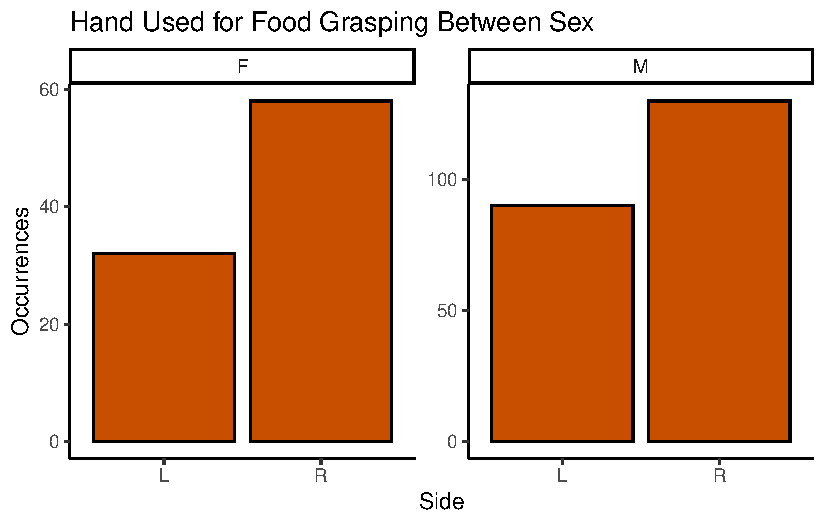
\includegraphics{LeftyLemurs_files/figure-pdf/unnamed-chunk-39-1.pdf}

}

\end{figure}

Trying some statistical tests

\begin{Shaded}
\begin{Highlighting}[]
\NormalTok{L }\SpecialCharTok{\%\textgreater{}\%} 
  \FunctionTok{group\_by}\NormalTok{(Side) }\SpecialCharTok{\%\textgreater{}\%} 
  \FunctionTok{summarise}\NormalTok{ (}\AttributeTok{n =} \FunctionTok{n}\NormalTok{()) }\SpecialCharTok{\%\textgreater{}\%}
  \FunctionTok{mutate}\NormalTok{(}\AttributeTok{proportion =}\NormalTok{ n }\SpecialCharTok{/} \FunctionTok{sum}\NormalTok{(n))}
\end{Highlighting}
\end{Shaded}

\begin{verbatim}
# A tibble: 2 x 3
  Side      n proportion
  <chr> <int>      <dbl>
1 L       257      0.413
2 R       365      0.587
\end{verbatim}

\begin{Shaded}
\begin{Highlighting}[]
\NormalTok{l\_handstuff }\SpecialCharTok{\%\textgreater{}\%} 
  \FunctionTok{group\_by}\NormalTok{(Side) }\SpecialCharTok{\%\textgreater{}\%} 
  \FunctionTok{summarise}\NormalTok{ (}\AttributeTok{n =} \FunctionTok{n}\NormalTok{()) }\SpecialCharTok{\%\textgreater{}\%}
  \FunctionTok{mutate}\NormalTok{(}\AttributeTok{proportion =}\NormalTok{ n }\SpecialCharTok{/} \FunctionTok{sum}\NormalTok{(n))}
\end{Highlighting}
\end{Shaded}

\begin{verbatim}
# A tibble: 2 x 3
  Side      n proportion
  <chr> <int>      <dbl>
1 L       218      0.417
2 R       305      0.583
\end{verbatim}

\begin{Shaded}
\begin{Highlighting}[]
\FunctionTok{binom.test}\NormalTok{(}\DecValTok{218}\NormalTok{, }\DecValTok{305}\NormalTok{, }\AttributeTok{p =}\NormalTok{ .}\DecValTok{75}\NormalTok{, }\AttributeTok{alternative =} \StringTok{"two.sided"}\NormalTok{)}
\end{Highlighting}
\end{Shaded}

\begin{verbatim}

    Exact binomial test

data:  218 and 305
number of successes = 218, number of trials = 305, p-value = 0.1648
alternative hypothesis: true probability of success is not equal to 0.75
95 percent confidence interval:
 0.6605189 0.7647621
sample estimates:
probability of success 
             0.7147541 
\end{verbatim}

Trying to do chi-squared test and contigency coefficients (did not work)

\begin{Shaded}
\begin{Highlighting}[]
\CommentTok{\# tbl\_handGrasps \textless{}{-} as.data.frame(l\_noLA) \%\textgreater{}\% }
  \CommentTok{\# group\_by(Side, Sex) \%\textgreater{}\% }
  \CommentTok{\# summarize(qty = sum(Freq)) \%\textgreater{}\% }
  \CommentTok{\# ungroup() \%\textgreater{}\% }
 \CommentTok{\#  spread(key = Sex, value = qty)}

\CommentTok{\# mat\_handGrasps \textless{}{-} as.matrix(tbl\_handGrasps[{-}1])}
\CommentTok{\# rownames(mat\_handGrasps) \textless{}{-} levels(tbl\_handGrasps$Side)}

\CommentTok{\# chisq.test(mat\_handGrasps)}
\end{Highlighting}
\end{Shaded}

It says it can't because it doesnt understand ``Freq''

\begin{Shaded}
\begin{Highlighting}[]
\FunctionTok{ggplot}\NormalTok{ (l\_grasps, }\FunctionTok{aes}\NormalTok{(}\AttributeTok{x=}\NormalTok{ Side)) }\SpecialCharTok{+}
  \FunctionTok{geom\_bar}\NormalTok{(}\AttributeTok{color =} \StringTok{"black"}\NormalTok{, }\AttributeTok{fill =} \StringTok{"\#C84E00"}\NormalTok{) }\SpecialCharTok{+}
  \FunctionTok{theme\_classic}\NormalTok{() }\SpecialCharTok{+}
  \FunctionTok{xlab}\NormalTok{(}\StringTok{"Left or Right Side"}\NormalTok{) }\SpecialCharTok{+}
  \FunctionTok{ylab}\NormalTok{(}\StringTok{"\# of Times Using Each Limb"}\NormalTok{) }\SpecialCharTok{+}
  \FunctionTok{ggtitle}\NormalTok{(}\StringTok{"Hand Use for Grasping Between Sexes"}\NormalTok{) }\SpecialCharTok{+}
  \FunctionTok{facet\_wrap}\NormalTok{ (}\SpecialCharTok{\textasciitilde{}}\NormalTok{ Sex, }\AttributeTok{scales =} \StringTok{"free"}\NormalTok{)}
\end{Highlighting}
\end{Shaded}

\begin{figure}[H]

{\centering 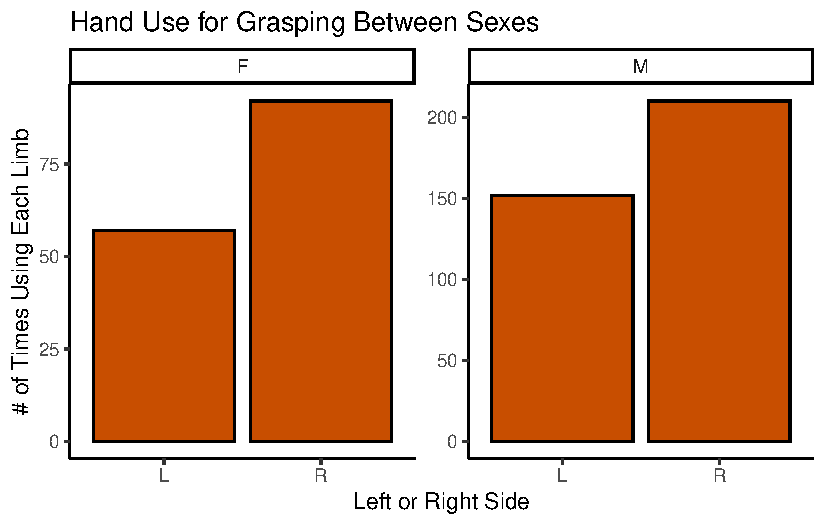
\includegraphics{LeftyLemurs_files/figure-pdf/unnamed-chunk-42-1.pdf}

}

\end{figure}

\begin{Shaded}
\begin{Highlighting}[]
\CommentTok{\#I echo: false}
\FunctionTok{ggplot}\NormalTok{ (L, }\FunctionTok{aes}\NormalTok{(}\AttributeTok{x=}\NormalTok{ Limb)) }\SpecialCharTok{+}
  \FunctionTok{geom\_bar}\NormalTok{(}\AttributeTok{color =} \StringTok{"black"}\NormalTok{, }\AttributeTok{fill =} \StringTok{"\#C84E00"}\NormalTok{) }\SpecialCharTok{+}
  \FunctionTok{theme\_classic}\NormalTok{() }\SpecialCharTok{+}
  \FunctionTok{xlab}\NormalTok{(}\StringTok{"Limb"}\NormalTok{) }\SpecialCharTok{+}
  \FunctionTok{ylab}\NormalTok{(}\StringTok{"\# of Times Using Each Limb"}\NormalTok{) }\SpecialCharTok{+}
  \FunctionTok{ggtitle}\NormalTok{(}\StringTok{"Limb Use Between Individuals"}\NormalTok{) }\SpecialCharTok{+}
  \FunctionTok{facet\_wrap}\NormalTok{ (}\SpecialCharTok{\textasciitilde{}}\NormalTok{ Focal)}
\end{Highlighting}
\end{Shaded}

\begin{figure}[H]

{\centering 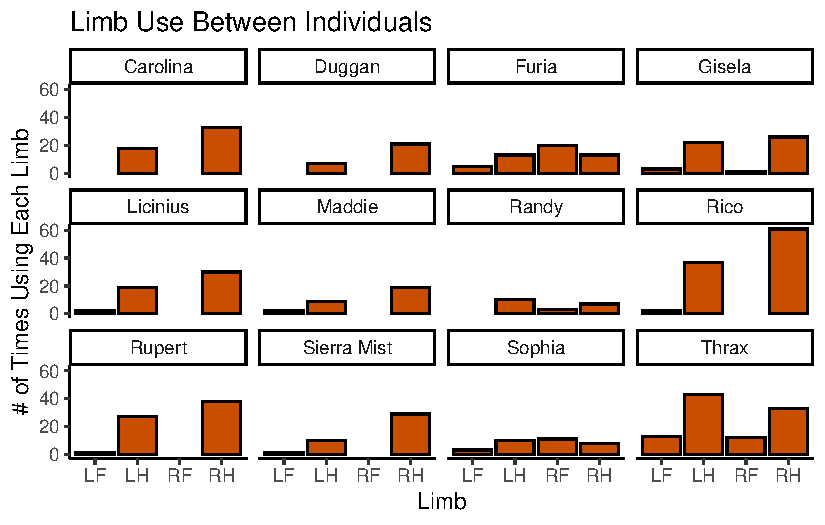
\includegraphics{LeftyLemurs_files/figure-pdf/unnamed-chunk-43-1.pdf}

}

\end{figure}

Not a lot of foot use. It might not be very useful to include these data

Just look at bipedal locomotion

\begin{Shaded}
\begin{Highlighting}[]
\NormalTok{l\_feet }\OtherTok{\textless{}{-}} 
\NormalTok{L }\SpecialCharTok{\%\textgreater{}\%} 
  \FunctionTok{filter}\NormalTok{(Category }\SpecialCharTok{==} \StringTok{"BP"}\NormalTok{)}

\FunctionTok{ggplot}\NormalTok{ (l\_feet, }\FunctionTok{aes}\NormalTok{(}\AttributeTok{x=}\NormalTok{ Limb)) }\SpecialCharTok{+}
  \FunctionTok{geom\_bar}\NormalTok{(}\AttributeTok{color =} \StringTok{"black"}\NormalTok{, }\AttributeTok{fill =} \StringTok{"\#C84E00"}\NormalTok{) }\SpecialCharTok{+}
  \FunctionTok{theme\_classic}\NormalTok{() }\SpecialCharTok{+}
  \FunctionTok{xlab}\NormalTok{(}\StringTok{"Limb"}\NormalTok{) }\SpecialCharTok{+}
  \FunctionTok{ylab}\NormalTok{(}\StringTok{"\# of Times Using Each Limb"}\NormalTok{) }\SpecialCharTok{+}
  \FunctionTok{ggtitle}\NormalTok{(}\StringTok{"Foot Use Between Individuals"}\NormalTok{) }\SpecialCharTok{+}
  \FunctionTok{facet\_wrap}\NormalTok{ (}\SpecialCharTok{\textasciitilde{}}\NormalTok{ Focal)}
\end{Highlighting}
\end{Shaded}

\begin{figure}[H]

{\centering 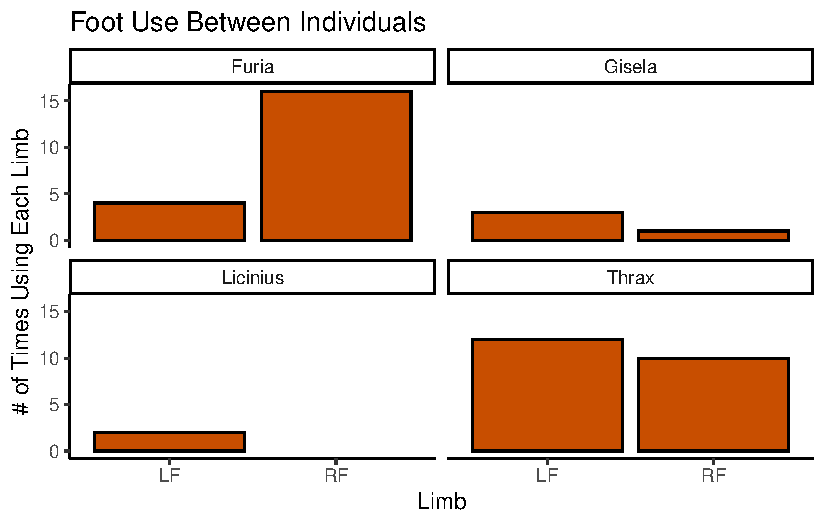
\includegraphics{LeftyLemurs_files/figure-pdf/unnamed-chunk-44-1.pdf}

}

\end{figure}

I don't really see any overall patterns here. It looks like Furia leads
with her right foor more than left and Thrax leads a little more with
his left foot than right.

Does age impact hand use?

\begin{Shaded}
\begin{Highlighting}[]
\FunctionTok{ggplot}\NormalTok{(L, }\FunctionTok{aes}\NormalTok{(}\AttributeTok{x =}\NormalTok{ Category, }\AttributeTok{y =}\NormalTok{ Age, }\AttributeTok{color =}\NormalTok{ Side)) }\SpecialCharTok{+} 
  \FunctionTok{geom\_jitter}\NormalTok{()  }\SpecialCharTok{+}
  \FunctionTok{theme\_classic}\NormalTok{() }\SpecialCharTok{+}
  \FunctionTok{xlab}\NormalTok{(}\StringTok{"Type of Behavior"}\NormalTok{) }\SpecialCharTok{+}
  \FunctionTok{ylab}\NormalTok{(}\StringTok{"Age of Lemur"}\NormalTok{) }\SpecialCharTok{+}
  \FunctionTok{ggtitle}\NormalTok{(}\StringTok{"Does Age Affect Limb Use?"}\NormalTok{) }\SpecialCharTok{+} 
  \FunctionTok{scale\_color\_manual}\NormalTok{(}\AttributeTok{values =} \FunctionTok{c}\NormalTok{(}\StringTok{"\#1D6363"}\NormalTok{, }\StringTok{"\#E89923"}\NormalTok{))}
\end{Highlighting}
\end{Shaded}

\begin{figure}[H]

{\centering 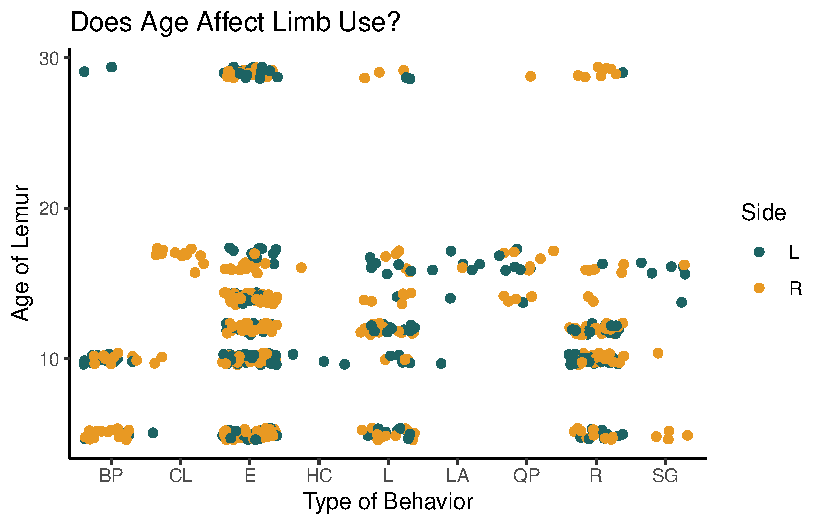
\includegraphics{LeftyLemurs_files/figure-pdf/unnamed-chunk-45-1.pdf}

}

\end{figure}

Yeah I don't think it does lol

Trying to make the graph I yearn for

\begin{Shaded}
\begin{Highlighting}[]
\FunctionTok{ggplot}\NormalTok{ (l\_noLA, }\FunctionTok{aes}\NormalTok{(}\AttributeTok{x=}\NormalTok{ Category, }\AttributeTok{fill =}\NormalTok{ Side)) }\SpecialCharTok{+}
  \FunctionTok{geom\_bar}\NormalTok{(}\AttributeTok{color =} \StringTok{"black"}\NormalTok{) }\SpecialCharTok{+}
  \FunctionTok{theme\_classic}\NormalTok{() }\SpecialCharTok{+}
  \FunctionTok{xlab}\NormalTok{(}\StringTok{"Type of Behavior"}\NormalTok{) }\SpecialCharTok{+}
  \FunctionTok{ylab}\NormalTok{(}\StringTok{"\# of Times Using Each Limb"}\NormalTok{) }\SpecialCharTok{+}
  \FunctionTok{ggtitle}\NormalTok{(}\StringTok{"Limb Use Between Lemur Species"}\NormalTok{) }\SpecialCharTok{+}
  \FunctionTok{facet\_wrap}\NormalTok{ (}\SpecialCharTok{\textasciitilde{}}\NormalTok{ Species, }\AttributeTok{scales =} \StringTok{"free"}\NormalTok{) }\SpecialCharTok{+} 
  \FunctionTok{scale\_fill\_manual}\NormalTok{(}\AttributeTok{values =} \FunctionTok{c}\NormalTok{(}\StringTok{"\#1D6363"}\NormalTok{, }\StringTok{"\#E89923"}\NormalTok{))}
\end{Highlighting}
\end{Shaded}

\begin{figure}[H]

{\centering 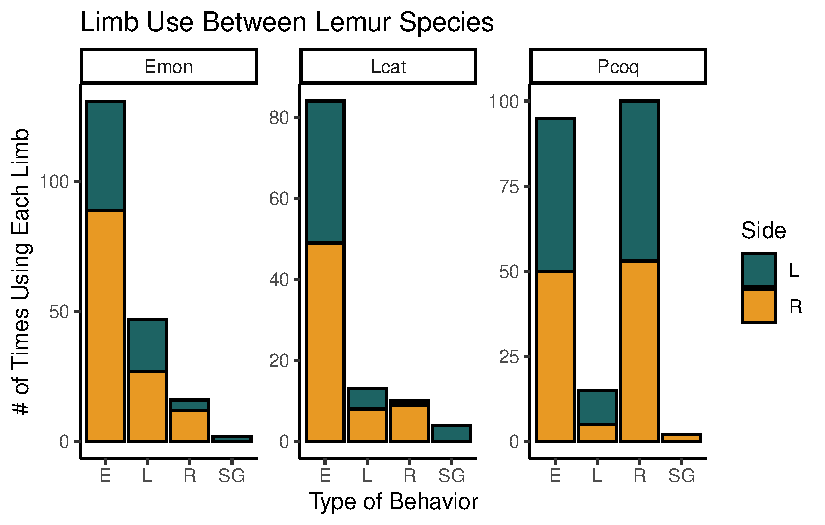
\includegraphics{LeftyLemurs_files/figure-pdf/unnamed-chunk-46-1.pdf}

}

\end{figure}

It's still not exactly what I want. I want the Y-axis to be \% of grasps
being with left hand, not total times used. Splitting by color makes it
really hard to read, but Idk how else to do it :P

\begin{Shaded}
\begin{Highlighting}[]
\FunctionTok{ggplot}\NormalTok{ (l\_noLA, }\FunctionTok{aes}\NormalTok{(}\AttributeTok{x=}\NormalTok{ Side, }\AttributeTok{fill =} \FunctionTok{interaction}\NormalTok{(Category, Side))) }\SpecialCharTok{+}
  \FunctionTok{geom\_bar}\NormalTok{(}\AttributeTok{color =} \StringTok{"black"}\NormalTok{) }\SpecialCharTok{+}
  \FunctionTok{theme\_classic}\NormalTok{() }\SpecialCharTok{+}
  \FunctionTok{xlab}\NormalTok{(}\StringTok{"Left or Right Side"}\NormalTok{) }\SpecialCharTok{+}
  \FunctionTok{ylab}\NormalTok{(}\StringTok{"\# of Times Using Each Limb"}\NormalTok{) }\SpecialCharTok{+}
  \FunctionTok{ggtitle}\NormalTok{(}\StringTok{"Limb Use Between Lemur Species"}\NormalTok{) }\SpecialCharTok{+}
  \FunctionTok{facet\_wrap}\NormalTok{ (}\SpecialCharTok{\textasciitilde{}}\NormalTok{ Species, }\AttributeTok{scales =} \StringTok{"free"}\NormalTok{)}
\end{Highlighting}
\end{Shaded}

\begin{figure}[H]

{\centering 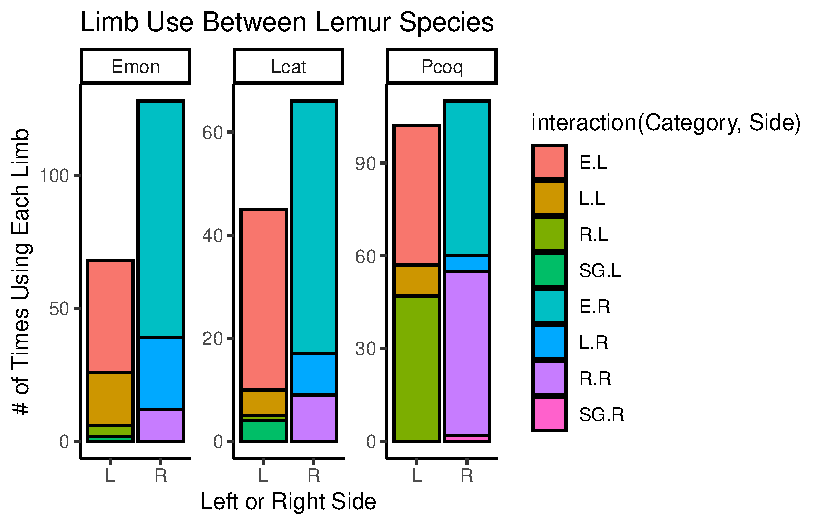
\includegraphics{LeftyLemurs_files/figure-pdf/unnamed-chunk-47-1.pdf}

}

\end{figure}

Wow that it was too complicated. Why did I dare make this monstrosity?

Okay, the landing and foot use data is fun and all, but the hand grasps
it what I actually need to look at. I'm going to make that into a .CSV
and analyze the data in JMP

\begin{Shaded}
\begin{Highlighting}[]
\CommentTok{\# write\_csv (l\_grasps, "HandGrasps.csv")}

\FunctionTok{summary}\NormalTok{(l\_grasps)}
\end{Highlighting}
\end{Shaded}

\begin{verbatim}
   Category            Troop              Focal             Species         
 Length:511         Length:511         Length:511         Length:511        
 Class :character   Class :character   Class :character   Class :character  
 Mode  :character   Mode  :character   Mode  :character   Mode  :character  
                                                                            
                                                                            
                                                                            
      Age            Sex                Month            Day       
 Min.   : 5.00   Length:511         Min.   :6.000   Min.   : 1.00  
 1st Qu.:10.00   Class :character   1st Qu.:6.000   1st Qu.: 8.00  
 Median :12.00   Mode  :character   Median :6.000   Median :22.00  
 Mean   :12.05                      Mean   :6.446   Mean   :18.19  
 3rd Qu.:14.00                      3rd Qu.:7.000   3rd Qu.:28.00  
 Max.   :29.00                      Max.   :7.000   Max.   :30.00  
      Year          Time               Side               Note          
 Min.   :2022   Length:511         Length:511         Length:511        
 1st Qu.:2022   Class :character   Class :character   Class :character  
 Median :2022   Mode  :character   Mode  :character   Mode  :character  
 Mean   :2022                                                           
 3rd Qu.:2022                                                           
 Max.   :2022                                                           
\end{verbatim}

\hypertarget{testing-significance}{%
\subsection{Testing significance:}\label{testing-significance}}

Species (significant)

\begin{Shaded}
\begin{Highlighting}[]
\FunctionTok{table}\NormalTok{(l\_grasps}\SpecialCharTok{$}\NormalTok{Side, l\_grasps}\SpecialCharTok{$}\NormalTok{Species)}
\end{Highlighting}
\end{Shaded}

\begin{verbatim}
   
    Emon Lcat Pcoq
  L   66   41  102
  R  128   66  108
\end{verbatim}

\begin{Shaded}
\begin{Highlighting}[]
\FunctionTok{chisq.test}\NormalTok{(}\FunctionTok{table}\NormalTok{(l\_grasps}\SpecialCharTok{$}\NormalTok{Side, l\_grasps}\SpecialCharTok{$}\NormalTok{Species))}
\end{Highlighting}
\end{Shaded}

\begin{verbatim}

    Pearson's Chi-squared test

data:  table(l_grasps$Side, l_grasps$Species)
X-squared = 9.2063, df = 2, p-value = 0.01002
\end{verbatim}

Sex (not significant)

\begin{Shaded}
\begin{Highlighting}[]
\FunctionTok{table}\NormalTok{(l\_grasps}\SpecialCharTok{$}\NormalTok{Side, l\_grasps}\SpecialCharTok{$}\NormalTok{Sex)}
\end{Highlighting}
\end{Shaded}

\begin{verbatim}
   
      F   M
  L  57 152
  R  92 210
\end{verbatim}

\begin{Shaded}
\begin{Highlighting}[]
\FunctionTok{chisq.test}\NormalTok{(}\FunctionTok{table}\NormalTok{(l\_grasps}\SpecialCharTok{$}\NormalTok{Side, l\_grasps}\SpecialCharTok{$}\NormalTok{Sex))}
\end{Highlighting}
\end{Shaded}

\begin{verbatim}

    Pearson's Chi-squared test with Yates' continuity correction

data:  table(l_grasps$Side, l_grasps$Sex)
X-squared = 0.46415, df = 1, p-value = 0.4957
\end{verbatim}

Focal (significant)

\begin{Shaded}
\begin{Highlighting}[]
\FunctionTok{table}\NormalTok{(l\_grasps}\SpecialCharTok{$}\NormalTok{Side, l\_grasps}\SpecialCharTok{$}\NormalTok{Focal)}
\end{Highlighting}
\end{Shaded}

\begin{verbatim}
   
    Carolina Duggan Furia Gisela Licinius Maddie Randy Rico Rupert Sierra Mist
  L       18      5    13     22       19      6     2   37     27          10
  R       33     18    12     25       29     16     6   61     38          27
   
    Sophia Thrax
  L     10    40
  R      4    33
\end{verbatim}

\begin{Shaded}
\begin{Highlighting}[]
\FunctionTok{chisq.test}\NormalTok{(}\FunctionTok{table}\NormalTok{(l\_grasps}\SpecialCharTok{$}\NormalTok{Side, l\_grasps}\SpecialCharTok{$}\NormalTok{Focal))}
\end{Highlighting}
\end{Shaded}

\begin{verbatim}
Warning in chisq.test(table(l_grasps$Side, l_grasps$Focal)): Chi-squared
approximation may be incorrect
\end{verbatim}

\begin{verbatim}

    Pearson's Chi-squared test

data:  table(l_grasps$Side, l_grasps$Focal)
X-squared = 23.257, df = 11, p-value = 0.01626
\end{verbatim}

Category (not significant)

\begin{Shaded}
\begin{Highlighting}[]
\FunctionTok{table}\NormalTok{(l\_grasps}\SpecialCharTok{$}\NormalTok{Side, l\_grasps}\SpecialCharTok{$}\NormalTok{Category)}
\end{Highlighting}
\end{Shaded}

\begin{verbatim}
   
      E   L   R
  L 122  35  52
  R 188  40  74
\end{verbatim}

\begin{Shaded}
\begin{Highlighting}[]
\FunctionTok{chisq.test}\NormalTok{(}\FunctionTok{table}\NormalTok{(l\_grasps}\SpecialCharTok{$}\NormalTok{Side, l\_grasps}\SpecialCharTok{$}\NormalTok{Category))}
\end{Highlighting}
\end{Shaded}

\begin{verbatim}

    Pearson's Chi-squared test

data:  table(l_grasps$Side, l_grasps$Category)
X-squared = 1.3451, df = 2, p-value = 0.5104
\end{verbatim}

Age (significant)

\begin{Shaded}
\begin{Highlighting}[]
\FunctionTok{table}\NormalTok{(l\_grasps}\SpecialCharTok{$}\NormalTok{Side, l\_grasps}\SpecialCharTok{$}\NormalTok{Age)}
\end{Highlighting}
\end{Shaded}

\begin{verbatim}
   
     5 10 12 14 16 17 29
  L 50 62 45 15  8 10 19
  R 73 58 71 45 22  4 29
\end{verbatim}

\begin{Shaded}
\begin{Highlighting}[]
\FunctionTok{chisq.test}\NormalTok{(}\FunctionTok{table}\NormalTok{(l\_grasps}\SpecialCharTok{$}\NormalTok{Side, l\_grasps}\SpecialCharTok{$}\NormalTok{Age))}
\end{Highlighting}
\end{Shaded}

\begin{verbatim}

    Pearson's Chi-squared test

data:  table(l_grasps$Side, l_grasps$Age)
X-squared = 20.193, df = 6, p-value = 0.002559
\end{verbatim}



\end{document}
